\documentclass[11pt,a4paper]{article}
\usepackage[a4paper,margin=18mm,headheight=22pt,footskip=16mm]{geometry}
\usepackage{fontspec}
\usepackage{unicode-math}
\setmathfont{STIX Math}
\setmainfont{DejaVu Sans}
\setsansfont{DejaVu Sans}
\setmonofont{DejaVu Sans Mono}
\usepackage[table]{xcolor}
\usepackage{graphicx}
\graphicspath{{../figures/}}
\usepackage{booktabs,longtable,tabularx,array,multirow}
\usepackage{enumitem}
\usepackage{fancyhdr}
\usepackage{titlesec}
\usepackage{tcolorbox}
\tcbuselibrary{breakable,skins}
\usepackage{xurl}
\usepackage{hyperref}
\usepackage{bookmark}
\usepackage{fancyvrb}
\usepackage{microtype}
\usepackage{caption}
\usepackage{float}
\usepackage{ragged2e}
\usepackage{amsmath}
\usepackage{calc}
\usepackage{lastpage}

\definecolor{UGTSNavy}{HTML}{0B1833}
\definecolor{UGTSNavyTwo}{HTML}{172744}
\definecolor{UGTSTeal}{HTML}{25B9B2}
\definecolor{UGTSCyan}{HTML}{5FD6E6}
\definecolor{UGTSBlue}{HTML}{6E8DF7}
\definecolor{UGTSPurple}{HTML}{9A78D8}
\definecolor{UGTSGold}{HTML}{E0B331}
\definecolor{UGTSCoral}{HTML}{E27266}
\definecolor{UGTSGreen}{HTML}{65C68B}
\definecolor{UGTSLight}{HTML}{F3F6FA}
\definecolor{UGTSMuted}{HTML}{66738A}
\definecolor{UGTSLine}{HTML}{D7DEE9}

\hypersetup{
  colorlinks=true,
  linkcolor=UGTSBlue,
  urlcolor=UGTSTeal,
  citecolor=UGTSPurple,
  pdftitle={UGTS Foundation 5.0 - Unicode Set-Field and Klein-Converse Atlas},
  pdfauthor={Prepared for Tom Klootwijk},
  pdfsubject={Content-addressed Unicode operators, signed set fields, Klein-converse parity and packed log-polar LUT execution},
  pdfkeywords={UGTS, Unicode, signed distance field, set theory, Klein bottle, SIMD, log-polar, operator atlas}
}

\pagestyle{fancy}
\fancyhf{}
\fancyhead[L]{\small\color{UGTSNavy}\textbf{UGTS FOUNDATION 5.0}}
\fancyhead[R]{\small\color{UGTSMuted}Unicode Set-Field and Klein-Converse Atlas}
\fancyfoot[L]{\small\color{UGTSMuted}Prepared for Tom Klootwijk - requester-supplied project attribution}
\fancyfoot[R]{\small\color{UGTSMuted}Page \thepage\ of \pageref*{LastPage}}
\renewcommand{\headrulewidth}{0.5pt}
\renewcommand{\headrule}{\hbox to\headwidth{\color{UGTSTeal}\leaders\hrule height \headrulewidth\hfill}}
\renewcommand{\footrulewidth}{0pt}

\titleformat{\section}{\Large\bfseries\color{UGTSNavy}}{\thesection}{0.6em}{}
\titleformat{\subsection}{\large\bfseries\color{UGTSTeal}}{\thesubsection}{0.5em}{}
\titleformat{\subsubsection}{\normalsize\bfseries\color{UGTSPurple}}{\thesubsubsection}{0.5em}{}
\titlespacing*{\section}{0pt}{18pt}{8pt}
\titlespacing*{\subsection}{0pt}{12pt}{5pt}

\setlist[itemize]{leftmargin=1.5em,itemsep=2.5pt,topsep=3pt}
\setlist[enumerate]{leftmargin=1.7em,itemsep=2.5pt,topsep=3pt}
\setlength{\parindent}{0pt}
\setlength{\parskip}{5pt}
\renewcommand{\arraystretch}{1.18}
\setlength{\tabcolsep}{4pt}

\newtcolorbox{decisionbox}[1][]{
  enhanced,breakable,colback=UGTSGreen!10,colframe=UGTSGreen!80!black,
  coltitle=white,fonttitle=\bfseries,title=FORMAL DECISION,
  boxed title style={colback=UGTSGreen!80!black},arc=1.5mm,boxrule=0.8pt,#1}
\newtcolorbox{evidencebox}[1][]{
  enhanced,breakable,colback=UGTSCoral!8,colframe=UGTSCoral!85!black,
  coltitle=white,fonttitle=\bfseries,title=EVIDENCE BOUNDARY,
  boxed title style={colback=UGTSCoral!85!black},arc=1.5mm,boxrule=0.8pt,#1}
\newtcolorbox{definitionbox}[1][]{
  enhanced,breakable,colback=UGTSPurple!7,colframe=UGTSPurple!90!black,
  coltitle=white,fonttitle=\bfseries,title=FORMAL DEFINITION,
  boxed title style={colback=UGTSPurple!90!black},arc=1.5mm,boxrule=0.8pt,#1}
\newtcolorbox{resultbox}[1][]{
  enhanced,breakable,colback=UGTSTeal!7,colframe=UGTSTeal!80!black,
  coltitle=white,fonttitle=\bfseries,title=VERIFIED RELEASE RESULT,
  boxed title style={colback=UGTSTeal!80!black},arc=1.5mm,boxrule=0.8pt,#1}
\newtcolorbox{boundarybox}[1][]{
  enhanced,breakable,colback=UGTSGold!9,colframe=UGTSGold!80!black,
  coltitle=UGTSNavy,fonttitle=\bfseries,title=BOUNDARY,
  boxed title style={colback=UGTSGold},arc=1.5mm,boxrule=0.8pt,#1}
\newtcolorbox{conclusionbox}[1][]{
  enhanced,breakable,colback=UGTSNavy,colframe=UGTSGold,
  coltext=white,coltitle=UGTSNavy,fonttitle=\bfseries,title=MAJOR-VERSION CONCLUSION,
  boxed title style={colback=UGTSGold},arc=1.8mm,boxrule=1.1pt,#1}

\newcolumntype{Y}{>{\RaggedRight\arraybackslash}X}
\newcolumntype{P}[1]{>{\RaggedRight\arraybackslash}p{#1}}
\newcommand{\source}[1]{\textcolor{UGTSPurple}{\textbf{[#1]}}}
\newcommand{\code}[1]{\texttt{\small #1}}
\newcommand{\status}[1]{\textbf{\textcolor{UGTSTeal}{#1}}}
\newcommand{\nonclaim}[1]{\textbf{\textcolor{UGTSCoral}{#1}}}

\begin{document}
\begin{titlepage}
\thispagestyle{empty}
\pagecolor{UGTSNavy}
\color{white}
\vspace*{6mm}
{\Large\color{UGTSCyan}\textbf{UNIFIED GEOMETRIC-TOPOLOGICAL SUBSTRATE}}\\[5mm]
{\fontsize{34}{39}\selectfont\textbf{UGTS FOUNDATION 5.0}}\\[4mm]
{\fontsize{21}{25}\selectfont\textbf{UNICODE SET-FIELD AND}}\\[1mm]
{\fontsize{21}{25}\selectfont\textbf{KLEIN-CONVERSE ATLAS}}\\[4mm]
{\large Content-addressed operator cells, signed set fields, reflective operand converse and packed log-polar execution}

\vspace{5mm}

\includegraphics[width=0.94\textwidth]{architecture.png}

\vfill
{\small\renewcommand{\arraystretch}{1.05}
\begin{tabularx}{\textwidth}{>{\bfseries\color{UGTSCyan}}P{43mm}Y}
Canonical identity & \code{ugts.foundation.unicode-set-field-klein-converse@5.0.0}\\
Legacy discovery alias & UGTS-KC 5.0\\
Component type & Foundation\\
Version / date & 5.0.0 / 29 August 2026\\
Codename & USF-KCA\\
Mechanism delta & USF001-USF064; legacy continuity M886-M949\\
Reference validation & 83 Python tests PASS; 3 schema instances with zero errors; C++20 scalar test PASS\\
Prepared for & Tom Klootwijk\\
\end{tabularx}}

\vspace{1.5mm}
\begin{tcolorbox}[colback=UGTSCoral!12!UGTSNavy,colframe=UGTSCoral,coltext=white,arc=1.5mm,boxrule=0.8pt,boxsep=1mm,left=1.5mm,right=1.5mm,top=1mm,bottom=1mm]
\footnotesize\textbf{ATTRIBUTION AND EVIDENCE BOUNDARY.} Requester-supplied attribution; technical artifact, not legal proof. Exact-SDF universality, finite mathematical completeness and physical SIMD performance are not claimed.
\end{tcolorbox}
\end{titlepage}
\nopagecolor
\color{black}

\pagenumbering{roman}
\section*{Executive Summary}
\addcontentsline{toc}{section}{Executive Summary}

\begin{decisionbox}
Release UGTS Foundation 5.0 as a component-scoped major version. The literal Unicode operator becomes the cold-atlas key for a content-addressed \emph{OperatorCell} that co-addresses exact Unicode spelling, typed syntax, semantic evaluator, canonical glyph SDF, signed set-field action, converse relation, Klein reflection rule, exactness capability, provenance and content hash. Geometry and semantics remain distinct typed faces; they are not collapsed into one notion of equality.
\end{decisionbox}

\begin{resultbox}
The accompanying package supplies 20 hash-verified OperatorCells; a 16-slot set-relation hot codebook with 14 assigned converse slots and two reserved slots; a corrected Packed Set-Field Node 32 codec; binary stream framing with CRC; a dependency-free Python reference runtime; portable C++20 scalar packing; an optional AVX2 extraction profile; JSON Schemas; a 64-mechanism delta; a 24-row claims ledger; runnable examples; a wheel; and captured validation evidence. The release test suite contains 83 passing Python tests. Three JSON instances validate with zero errors, and the native scalar codec test passes.
\end{resultbox}

\begin{conclusionbox}
A Unicode operator is no longer merely text and no longer merely an icon. It is a content-addressed, executable geometric rule cell whose literal codepoint resolves both its canonical shape and its typed operation. A Klein-converse parity flip mirrors the shape, reverses the typed ports and selects the converse Unicode spelling while preserving the mathematical truth value.
\end{conclusionbox}

\begin{evidencebox}
The immediate source document correctly identifies \texttt{∋} as the converse spelling of \texttt{∈}, proposes geometric operator primitives, log-polar fixed-point packing, a 32-bit node and SIMD decoding. It also contains packing errors, overloaded parity, incomplete geometry, and unsupported universal compression, speed, randomness and physical claims. Version 5.0 does not silently clean the source into a fictional proof. Every major claim is admitted, corrected, bounded or rejected in the machine-readable claims ledger. \source{S0}
\end{evidencebox}

\tableofcontents
\clearpage
\pagenumbering{arabic}

\section{Major Release Identity and Scope}
\subsection{Why this is a major version}
Version 5.0 changes the unit of formal operator identity. Earlier releases already established content-addressed definitions, representation profiles, log-polar packing, explicit reflective topology, general typed operators and field-capability boundaries. This release unifies those commitments in a new foundation component whose central object is the Unicode-addressed executable operator cell.

The major change is not a larger list of symbols. It is a stronger invariant:
\begin{quote}
\textbf{The exact Unicode literal is a stable lookup key into one record that carries syntax, typed semantics, canonical geometry, field behavior, converse topology and execution metadata.}
\end{quote}

A change in font outline does not silently change set membership. A change in operand spelling from \(x\in A\) to \(A\ni x\) does not create a second mathematical relation. A packed four-bit slot does not replace the global Unicode identity. These distinctions now belong to the formal release schema rather than explanatory prose.

\subsection{Component-scoped identity}
The versioning charter deprecates a single global ladder because compute profiles, foundations, runtimes, formal packs, applications and platform builds are not globally comparable. Version 5.0 therefore uses the canonical identity
\[
\texttt{ugts.foundation.unicode-set-field-klein-converse@5.0.0}.
\]
The legacy alias \textbf{UGTS-KC 5.0} remains for discovery. The parent graph records exactly which releases contribute architecture; it does not claim that this foundation supersedes unrelated game, scanner, solver or device branches. \source{S7}

\begin{figure}[H]
\centering
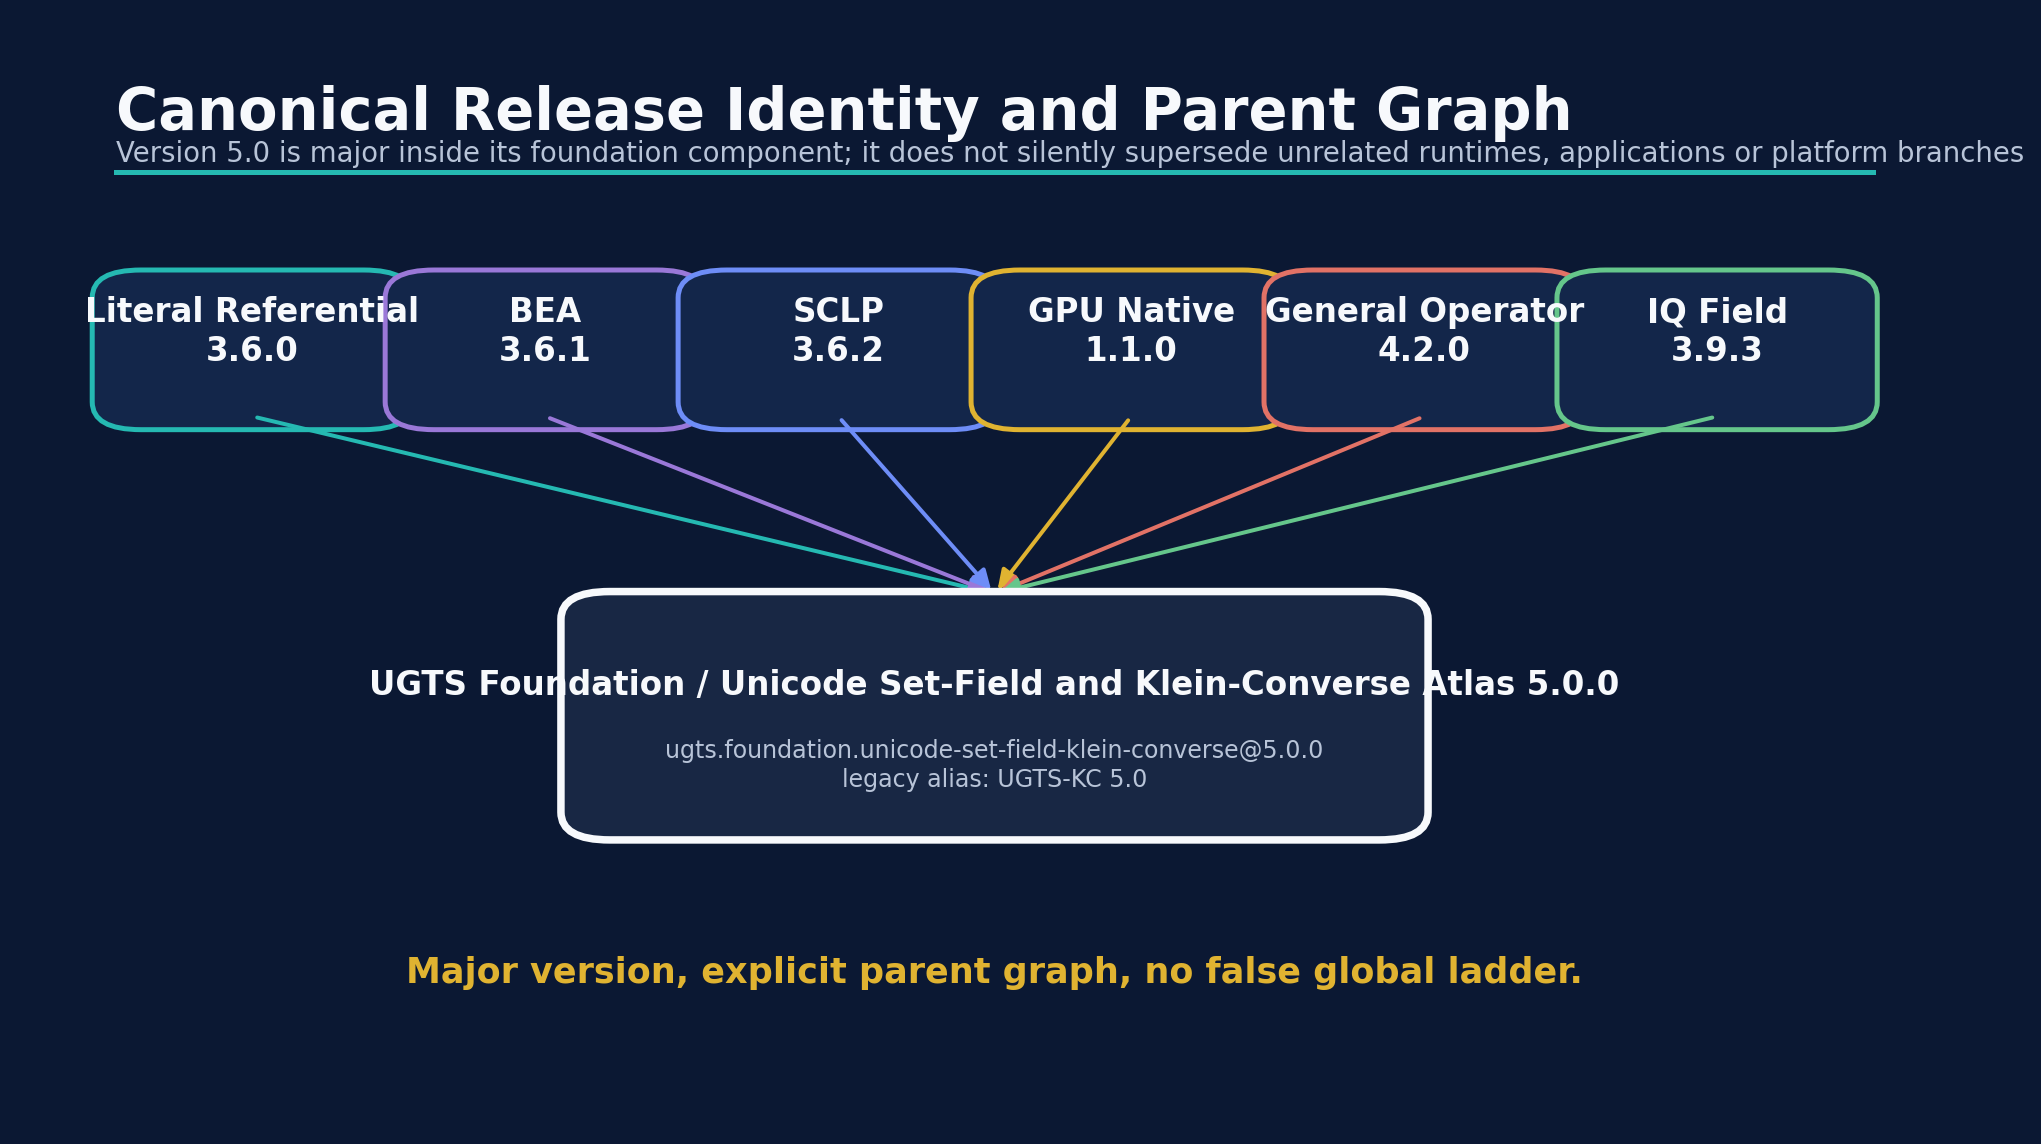
\includegraphics[width=0.98\textwidth]{release_parent_graph.png}
\caption{Version 5.0 is major within its foundation component. Typed parent edges replace a false global sequence.}
\end{figure}

\subsection{What 5.0 adds}
\begin{itemize}
\item A content-addressed \textbf{Unicode OperatorCell} schema.
\item A six-level signed set-field capability ladder.
\item Canonical set algebra over sign-compatible fields.
\item Direct/converse Unicode relation families with explicit surface-to-canonical port maps.
\item A reflective \textbf{Klein-converse involution}: operator converse, operand swap, chart reflection, orientation flip and \(\kappa\)-toggle.
\item A canonical capsule-union glyph SDF profile plus a font-exact profile boundary.
\item A cold Unicode atlas and a hash-bound hot 16-slot codebook.
\item A corrected 32-bit packed node and mandatory stream header.
\item Scalar, AVX2 and NEON execution contracts with a scalar oracle.
\item Exactness, quantization, integrity and event-margin certificates.
\item 64 new mechanisms and a complete claims ledger.
\end{itemize}

\subsection{What remains unchanged}
The canonical UGTS authority order is preserved:
\[
\text{support}\rightarrow\text{compatibility}\rightarrow\text{guard}\rightarrow
\text{verified proposal}\rightarrow\text{deterministic commit}\rightarrow\text{lineage}.
\]
Pure operator evaluation may produce evidence or a proposal. It cannot mutate authoritative state, topology, ownership or lineage by itself. Projection, glyph rendering, SIMD layout and packed storage remain replaceable implementations around the authority chain. \source{S4} \source{S5}

\section{Source Basis and Evidence Discipline}
\subsection{Registered sources}
\small
\rowcolors{2}{UGTSLight}{white}
\begin{longtable}{P{7mm}P{47mm}P{34mm}P{67mm}}
\toprule
\textbf{ID} & \textbf{Source} & \textbf{SHA-256 prefix} & \textbf{Use in 5.0}\\
\midrule
\endfirsthead
\toprule
\textbf{ID} & \textbf{Source} & \textbf{SHA-256 prefix} & \textbf{Use in 5.0}\\
\midrule
\endhead
\bottomrule
\endlastfoot
% BEGIN GENERATED source_table
S0 & \nolinkurl{mandible-broad-set-math-operator-CE-logo-like-simd256.pdf} & \texttt{6149e3d398c2...} & Immediate Unicode/SDF/log-polar/SIMD source motif \\
S1 & \nolinkurl{UGTS_KC_3_6_Tom_Klootwijk.pdf} & \texttt{e21433cd8378...} & Literal content-addressed definitions and operation order \\
S2 & \nolinkurl{UGTS_KC_3_6_1_BEA_Tom_Klootwijk.pdf} & \texttt{ac857c9c01f5...} & Representation profile, glyph SDF and typed semantic evaluator separation \\
S3 & \nolinkurl{UGTS_KC_3_6_2_SCLP_Tom_Klootwijk.pdf} & \texttt{6987490a0a7b...} & Log-polar chart, finite packing, half-turn/Klein distinction \\
S4 & \nolinkurl{Unified_Geometric_Topological_Substrate_GPU_Native_Addendum.pdf} & \texttt{3a6b6c57118c...} & Packed-state, one-bit and hardware evidence discipline \\
S5 & \nolinkurl{UGTS_KC_4_2_General_Operator_Order_Addendum(1).pdf} & \texttt{413ef9568330...} & General typed operator record and explicit order calculus \\
S6 & \nolinkurl{UGTS_KC_3_9_3_IQ_Field_Substrate_Tom_Klootwijk(1).pdf} & \texttt{c0ae58652436...} & Field exactness/capability and sign-preserving CSG boundary \\
S7 & \nolinkurl{UGTS_Versioning_Charter_Phase_1_Foundation_Chronology(1).pdf} & \texttt{1b64495ed32a...} & Component-scoped canonical identity and filename rule \\
% END GENERATED source_table
\end{longtable}
\normalsize

\subsection{Immediate source dissection}
The immediate source contributes five technically useful motifs:
\begin{enumerate}
\item \texttt{∈} and \texttt{∋} are converse surface spellings of one membership relation.
\item Unicode operator shapes can be described by bounded geometric primitives.
\item local geometry can be addressed in log-polar coordinates and packed into fixed-width records.
\item a one-bit selector can choose between declared orientations or relation directions.
\item SIMD extraction can decode several packed words in parallel.
\end{enumerate}

It also requires explicit correction:
\begin{itemize}
\item The source's example LUT selects codepoints by quadrant rather than evaluating the advertised glyph SDFs.
\item One packing expression overlaps angle and codepoint bits.
\item The proposed 32-bit decoder extracts the parity bit but does not verify payload parity.
\item The active bit is omitted by one unpacker.
\item A Boolean value of 0 or 1 is not a valid full byte/lane mask for \texttt{blendv}; it must be expanded.
\item A deterministic parity bit is not true randomness, anti-aliasing proof, complete state or cryptographic entropy.
\item A half-turn rotation is not an orientation-reversing Klein gluing.
\item Universal 16 KB, constant-time, cycle-count and collision-free-path claims are not established.
\end{itemize}

\subsection{Inherited commitments}
\textbf{Literal referential 3.6.0} makes definitions first-class, content-addressed substrate data with resolvable dependencies and explicit evaluation order. \source{S1}

\textbf{BEA 3.6.1} defines a representation profile containing normalization, glyph renderer, byte encoder and typed semantic evaluator. It insists that glyph SDF, semantic residual and encoding alignment remain separate spaces. Version 5.0 adopts that separation but lets one Unicode cell co-address all three. \source{S2}

\textbf{SCLP 3.6.2} supplies the log-polar chart and the decisive distinction between a source half-turn bundle and a genuine reflective Klein profile:
\[
(\rho,\theta,\varphi,o)\mapsto(\rho',\pi-\theta,-\varphi,-o).
\]
The angular derivative is \(-1\), so the base gluing reverses orientation. \source{S3}

\textbf{GPU Native 1.1} supplies the compact-state, narrow-one-bit, compression and hardware-evidence boundaries. \source{S4}

\textbf{General Operator and Order 4.2} supplies the typed OperatorSpec, explicit order profiles, exactness/effect/capability metadata and the rule that pure evaluation cannot bypass event authority. \source{S5}

\textbf{IQ Field 3.9.3} supplies the capability distinction between exact distance, conservative bounds and sign-correct residuals, including the warning that min/max CSG generally preserves sign but not exact Euclidean distance. \source{S6}

\subsection{Evidence classes}
\begin{tabularx}{\textwidth}{P{34mm}Y}
\toprule
\textbf{Class} & \textbf{Treatment in 5.0}\\
\midrule
Source-derived motif & Unicode converse, geometric glyph proposal, log-polar packing, branchless selector and SIMD sketch are registered as source motifs.\\
Engineering-derived & OperatorCell schema, signed set-field calculus, canonical capsule glyphs, Klein-converse transform, codebook and codecs are new formalization.\\
Measured package evidence & Tests, hashes, schema results, binary round trips, wheel and native scalar outputs are captured in \texttt{validation/}.\\
Bounded hypothesis & AVX2/NEON speed, cache behavior and target-device advantage remain benchmark questions.\\
Rejected claim & Universality, infinite detail, true randomness, automatic collision freedom and physical spacetime assertions are excluded.\\
\bottomrule
\end{tabularx}

\section{Formal 5.0 Architecture}
\subsection{Upgraded world object}
\begin{definitionbox}
Let the version-5 foundation object be
\[
W_{5}=W_{\mathrm{retained}}+(\mathcal{U},\mathcal{O},\Phi,\Gamma,\mathcal{K},\mathcal{C},\mathcal{P},\mathrm{Cert}),
\]
where \(\mathcal{U}\) is the Unicode literal domain; \(\mathcal{O}\) the content-addressed OperatorCell atlas; \(\Phi\) the signed set-field calculus; \(\Gamma\) canonical glyph fields; \(\mathcal{K}\) the Klein-converse transform; \(\mathcal{C}\) hot codebooks; \(\mathcal{P}\) packed execution records; and \(\mathrm{Cert}\) exactness, integrity, quantization and event-margin certificates.
\end{definitionbox}

\subsection{Canonical processing path}
\begin{Verbatim}[fontsize=\small,frame=single]
literal Unicode sequence
 -> normalize under declared profile
 -> resolve OperatorCell + content hash
 -> map surface operands to canonical typed ports
 -> evaluate semantic relation / set-field transform
 -> evaluate optional canonical glyph SDF
 -> apply optional Klein-converse chart transition
 -> resolve hot codebook slot
 -> pack or decode bounded execution record
 -> issue capability + error + integrity certificate
 -> support -> compatibility -> guard -> verified proposal
 -> deterministic commit -> lineage / replay
 -> optional render, storage, SIMD or device adapter
\end{Verbatim}

\begin{figure}[H]
\centering
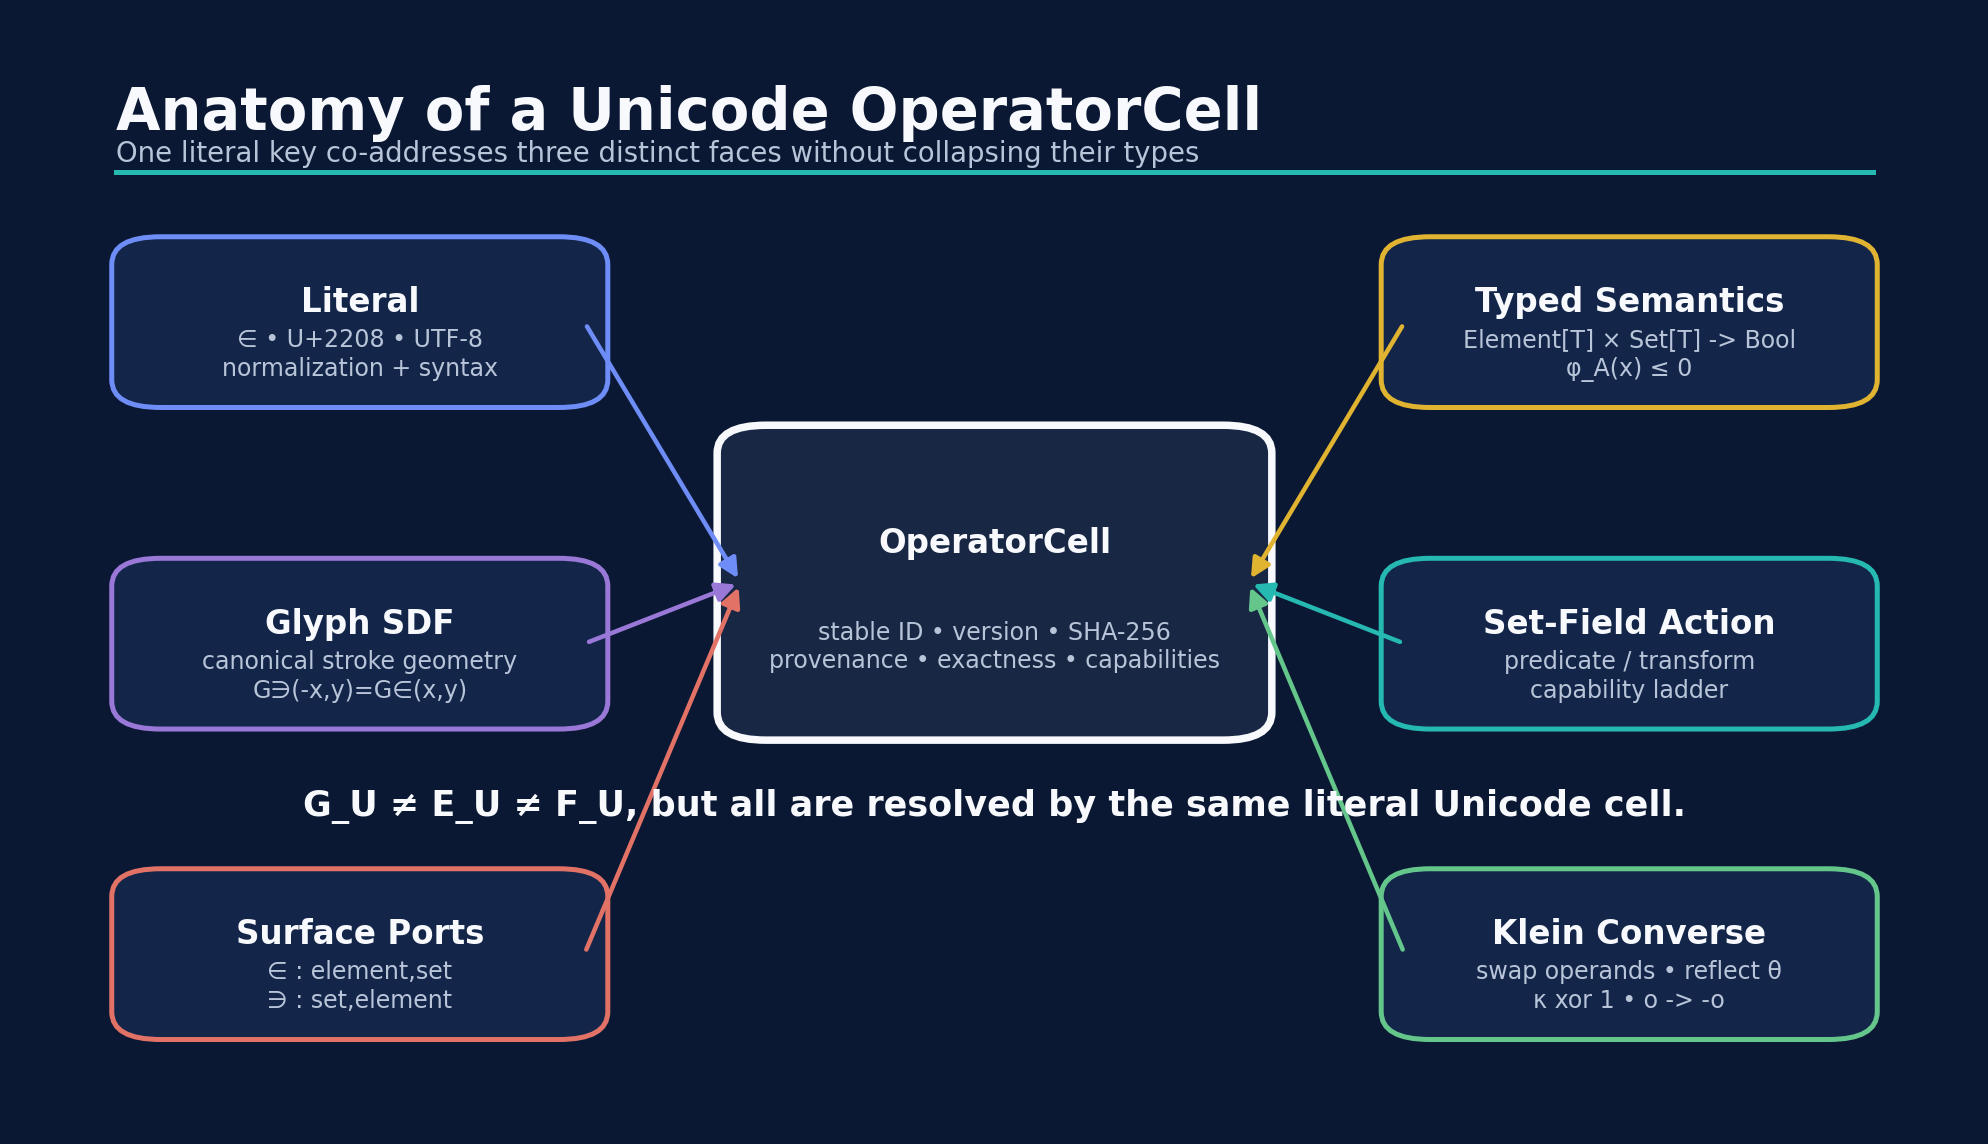
\includegraphics[width=\textwidth]{operator_cell.png}
\caption{The literal, glyph, semantics and field action are distinct but co-addressed.}
\end{figure}

\subsection{Single source of operator truth}
The same OperatorCell records feed schema validation, Unicode lookup, relation evaluation, glyph generation, converse mapping, hot-codebook construction, content hashing, report tables and tests. A prose-only operator meaning cannot override the machine-readable record.

\section{The Unicode OperatorCell}
\subsection{Formal record}
\begin{definitionbox}
For exact Unicode scalar sequence \(U\), define
\[
\mathcal{O}_{U}=(U,\ell_U,G_U,E_U,F_U,C_U,K_U,P_U,h_U),
\]
where \(\ell_U\) is the literal spelling; \(G_U\) canonical glyph SDF; \(E_U\) typed semantic evaluator; \(F_U\) set-field action; \(C_U\) typed ports and surface order; \(K_U\) converse/topology rule; \(P_U\) representation and exactness profile; and \(h_U\) the canonical content hash.
\end{definitionbox}

The record stored in \texttt{spec/operator\_atlas.json} additionally carries a stable ID, version, provenance, Unicode names, UTF-8 bytes, laws, capabilities and explicit non-claims.

\subsection{Literal identity}
The cold-atlas key is the exact NFC-normalized scalar sequence, not a font outline and not a short local opcode. For \(∈\):\par\smallskip
\begin{tabularx}{\textwidth}{P{42mm}Y}
\toprule
Literal & ∈\\
Unicode scalar & U+2208\\
Unicode name & ELEMENT OF\\
UTF-8 bytes & \texttt{e2 88 88}\\
Stable operator ID & \texttt{set.membership.element-of}\\
\bottomrule
\end{tabularx}

Compatibility normalization is deliberately not applied because it can collapse presentation-distinct mathematical symbols. A profile may register an alias, but the alias must point to a stable operator identity rather than silently replacing the literal.

\subsection{Typed ports and reversed operand order}
For membership, the canonical semantic ports are
\[
[\mathrm{element},\mathrm{container}].
\]
The two surface forms are
\[
x\in A \qquad\text{and}\qquad A\ni x.
\]
The direct syntax map is \([0,1]\); the converse syntax map is \([1,0]\). Both call one membership kernel after port normalization. This makes operand reversal executable data rather than a parser special case.

\subsection{Three faces, one address}
The release enforces
\[
G_U\neq E_U\neq F_U,
\]
yet resolves all three through the same literal cell. A glyph sample does not decide membership. A semantic truth value does not imply zero geometric glyph distance. A set-field transform does not establish a font's outline. The co-addressing is a referential convenience with typed boundaries, not a claim of cross-domain identity. \source{S2}

\subsection{Content addressing}
Each cell hash is computed from canonical UTF-8 JSON with sorted keys, NFC strings and no non-finite numbers, excluding only the hash field itself. The atlas hash commits to all cells and atlas metadata. A codebook commits to the atlas hash and each occupied operator-cell hash.

\begin{boundarybox}
A SHA-256 content address identifies bytes under the canonicalization policy. It is not legal authorship, ownership, priority, semantic truth or collision-free identity across every possible future policy.
\end{boundarybox}

\section{Set Theory as Signed Set Fields}
\subsection{General metric definition}
Let \(X\) be a declared universe with metric or graph distance \(d\), and \(A\subseteq X\). Define
\[
\phi_A(x)=d(x,A)-d(x,X\setminus A).
\]
Then, under the declared boundary policy,
\[
\phi_A(x)<0\ \text{inside},\qquad
\phi_A(x)=0\ \text{on the boundary},\qquad
\phi_A(x)>0\ \text{outside}.
\]
Membership becomes
\[
x\in A\iff\phi_A(x)\le 0.
\]

The definition is exact only when the metric and the representations of \(A\) and its complement are exact. Sampled point sets generally produce an approximation or bound rather than an exact continuous SDF.

\subsection{Finite and symbolic fallback}
When no useful metric exists, a signed characteristic field is sufficient:
\[
\chi_A(x)=\begin{cases}-1,&x\in A,\\+1,&x\notin A.\end{cases}
\]
The reference runtime implements \texttt{FiniteSetField} over a declared ordered finite universe. Its capability is \texttt{signed\_membership\_field}, not \texttt{exact\_sdf}.

\begin{figure}[H]
\centering
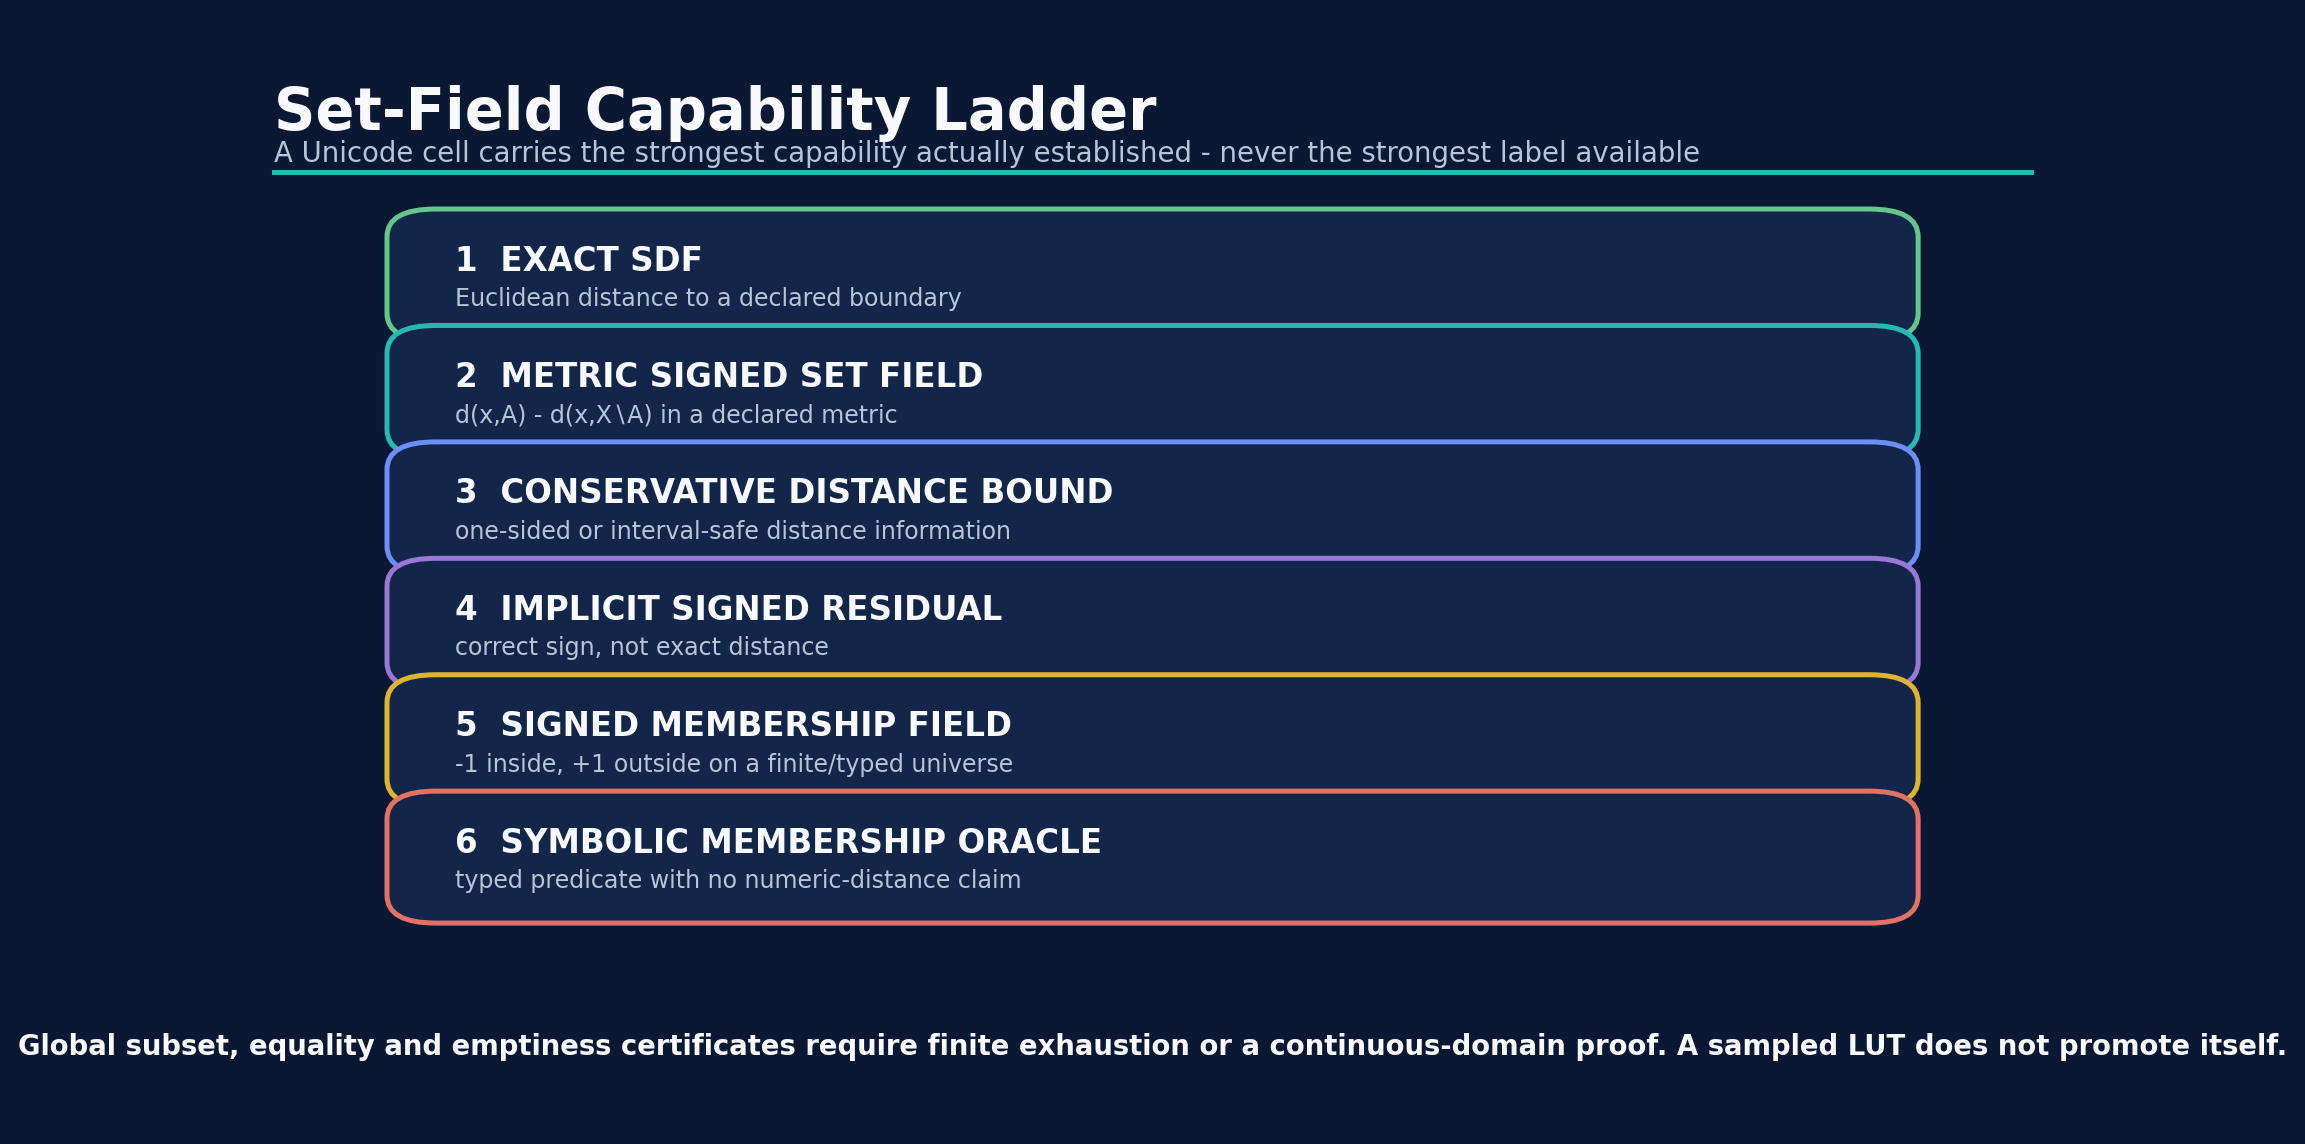
\includegraphics[width=\textwidth]{exactness_ladder.png}
\caption{Every field carries the strongest capability actually established.}
\end{figure}

\subsection{Set algebra as field algebra}
With the negative-inside convention:
\begin{align*}
\phi_{A\cup B}&=\min(\phi_A,\phi_B),\\
\phi_{A\cap B}&=\max(\phi_A,\phi_B),\\
\phi_{X\setminus A}&=-\phi_A,\\
\phi_{A\setminus B}&=\max(\phi_A,-\phi_B),\\
\phi_{A\triangle B}&=\max\!\left(\min(\phi_A,\phi_B),-\max(\phi_A,\phi_B)\right).
\end{align*}
These formulas preserve the correct inside/outside sign. They do not automatically preserve exact Euclidean distance after composition. \source{S6}

\begin{figure}[H]
\centering
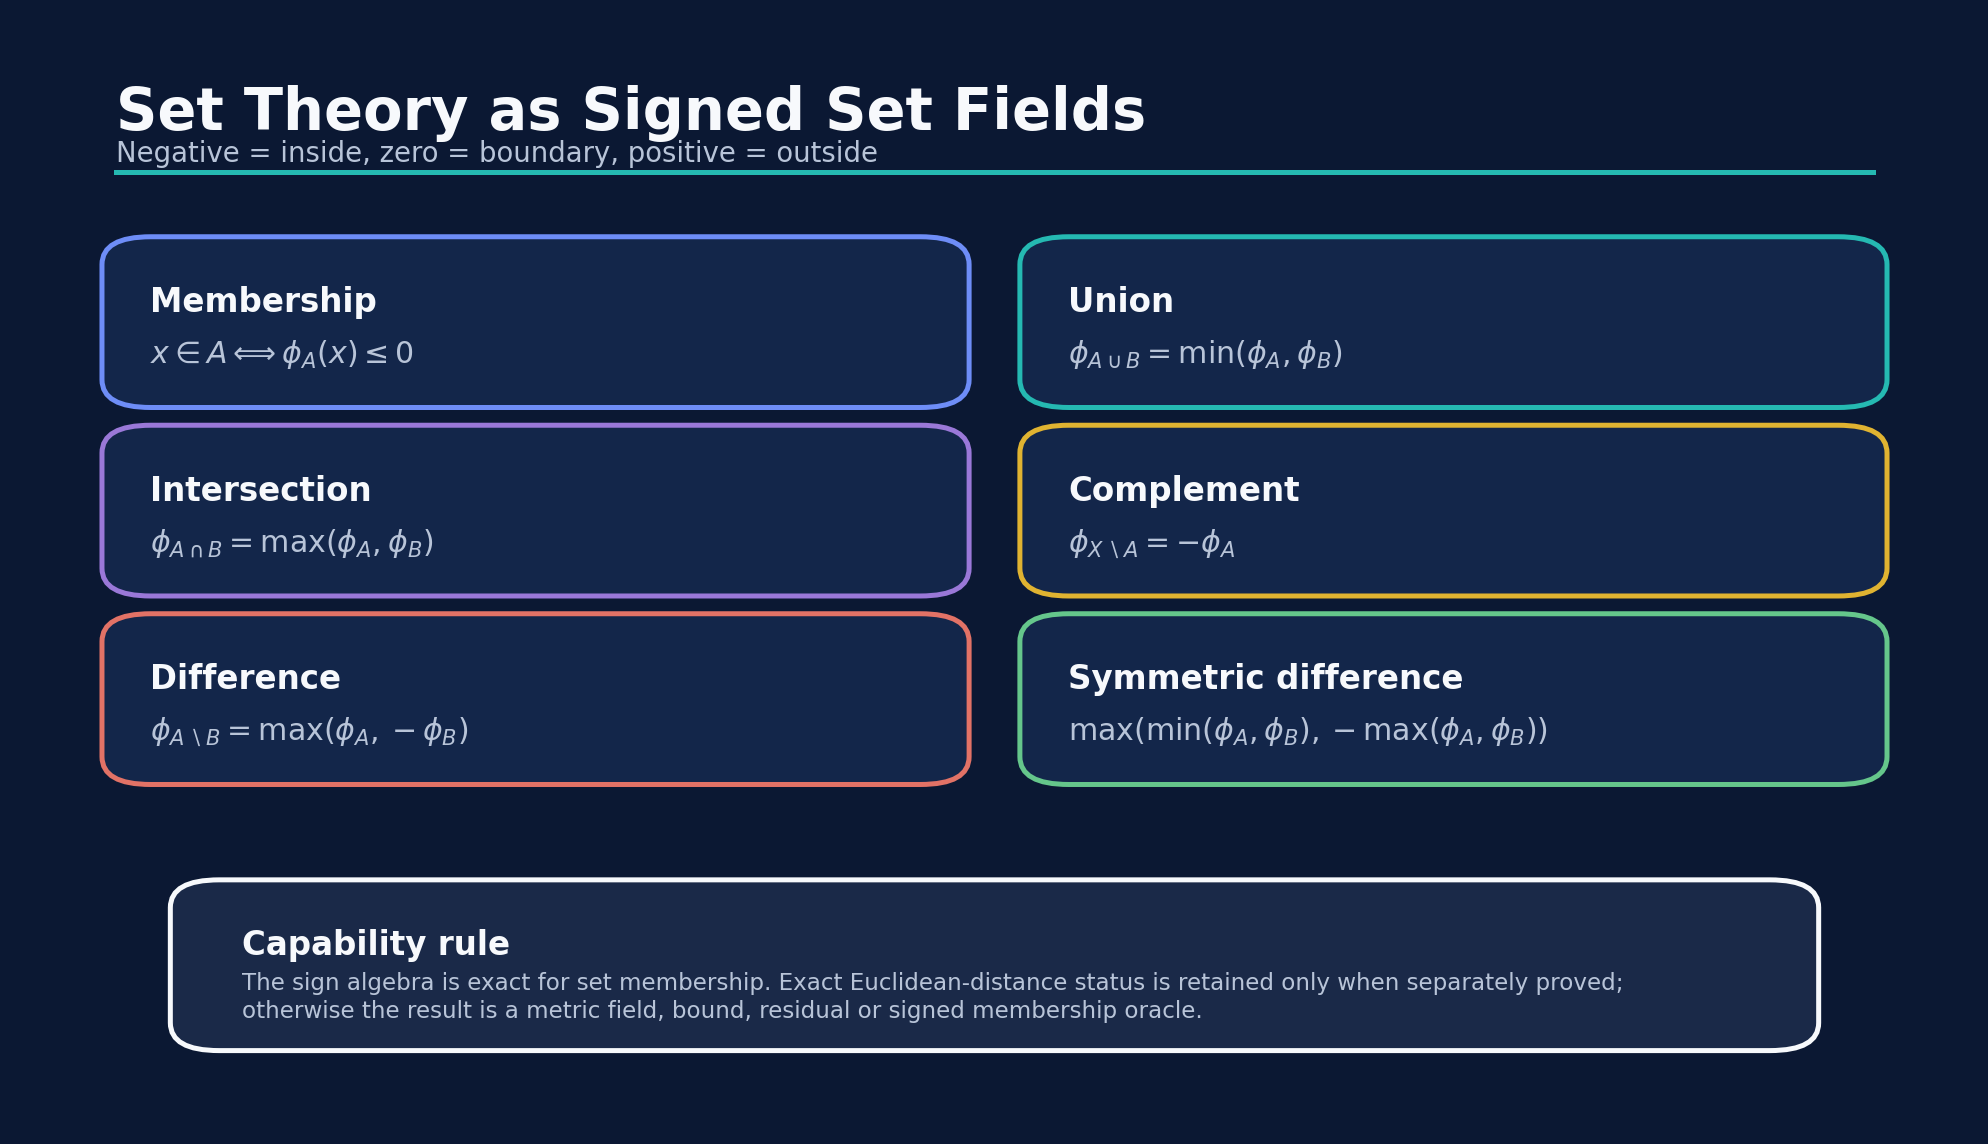
\includegraphics[width=\textwidth]{set_field_algebra.png}
\caption{The field layer turns set operations into bounded, branch-friendly scalar operations.}
\end{figure}

\subsection{Relation kernels}
The shipped reference subset implements:
\begin{align*}
x\in A &\iff \phi_A(x)\le 0,\\
x\notin A &\iff \phi_A(x)>0,\\
A\subseteq B &\iff A\setminus B=\varnothing,\\
A\subset B &\iff A\subseteq B\ \wedge\ A\ne B,\\
A=B &\iff A\subseteq B\ \wedge\ B\subseteq A.
\end{align*}
On a finite universe these statements may be checked exhaustively. On a continuous universe, a sampled LUT is not a universal emptiness or inclusion proof.

\subsection{Capability-aware certificates}
A set-field result carries at least:
\begin{itemize}
\item universe/profile identity;
\item sign convention and boundary inclusion policy;
\item capability class;
\item metric or oracle identity;
\item numeric error or interval;
\item proof scope: point query, finite exhaustive domain, sampled domain or continuous certificate;
\item explicit non-claims.
\end{itemize}

\section{Unicode Converse Families}
\subsection{Family plus \texorpdfstring{\(\kappa\)}{kappa}}
Each hot relation family uses
\[
\mathrm{operator\_id}=(\mathrm{family}\ll 1)\;|\;\kappa,
\qquad \kappa\in\{0,1\}.
\]
The family selects the canonical semantic relation. \(\kappa=0\) selects the direct spelling; \(\kappa=1\) selects the converse spelling and reversed surface ports.

\begin{tabularx}{\textwidth}{P{22mm}P{35mm}P{35mm}Y}
\toprule
\textbf{Family} & \(\kappa=0\) & \(\kappa=1\) & \textbf{Canonical relation}\\
\midrule
0 & \(x\in A\) & \(A\ni x\) & membership\\
1 & \(x\notin A\) & \(A\not\ni x\) & nonmembership\\
2 & \(A\subset B\) & \(B\supset A\) & proper inclusion\\
3 & \(A\subseteq B\) & \(B\supseteq A\) & inclusion or equality\\
4 & \(A\not\subset B\) & \(B\not\supset A\) & negated proper inclusion\\
5 & \(A\nsubseteq B\) & \(B\nsupseteq A\) & negated inclusion or equality\\
6 & \(A\subsetneq B\) & \(B\supsetneq A\) & strict-inclusion glyph variant\\
7 & reserved & reserved & codebook extension gate\\
\bottomrule
\end{tabularx}

\subsection{Semantic converse law}
For every registered pair \(U,U^{\smile}\),
\[
E_{U^{\smile}}(b,a)=E_U(a,b).
\]
This is relation converse, not functional inversion. Typed endpoints swap; multiplicity, provenance and truth are preserved.

\subsection{Algebra operators outside the hot pair codebook}
The cold atlas also ships \texttt{∪}, \texttt{∩}, \(\setminus\), \texttt{∁}, \texttt{∅} and \texttt{=}. They are addressed by Unicode and carry geometry plus functionality, but they do not consume a direct/converse slot in the shipped \texttt{set-core-16} codebook. A later codebook may assign them local slots without changing their global identities.

\section{The Klein-Converse Involution}
\subsection{Local transform}
Define the local transform
\[
\mathcal{K}(U,a,b,\rho,\theta,\kappa,o)
=\left(U^{\smile},b,a,\rho,\pi-\theta,\kappa\oplus1,-o\right).
\]
It acts simultaneously on literal spelling, typed ports, glyph orientation, chart angle and orientation state.

\subsection{Local involution and lineage}
On the local fiber,
\[
\mathcal{K}^{2}=\mathrm{id}.
\]
After two applications the literal, ports, angle, \(\kappa\) and orientation return. Lineage does \emph{not} erase the two wraps; the winding counter increases by two. Thus the state transform is involutive while history remains auditable.

\begin{figure}[H]
\centering
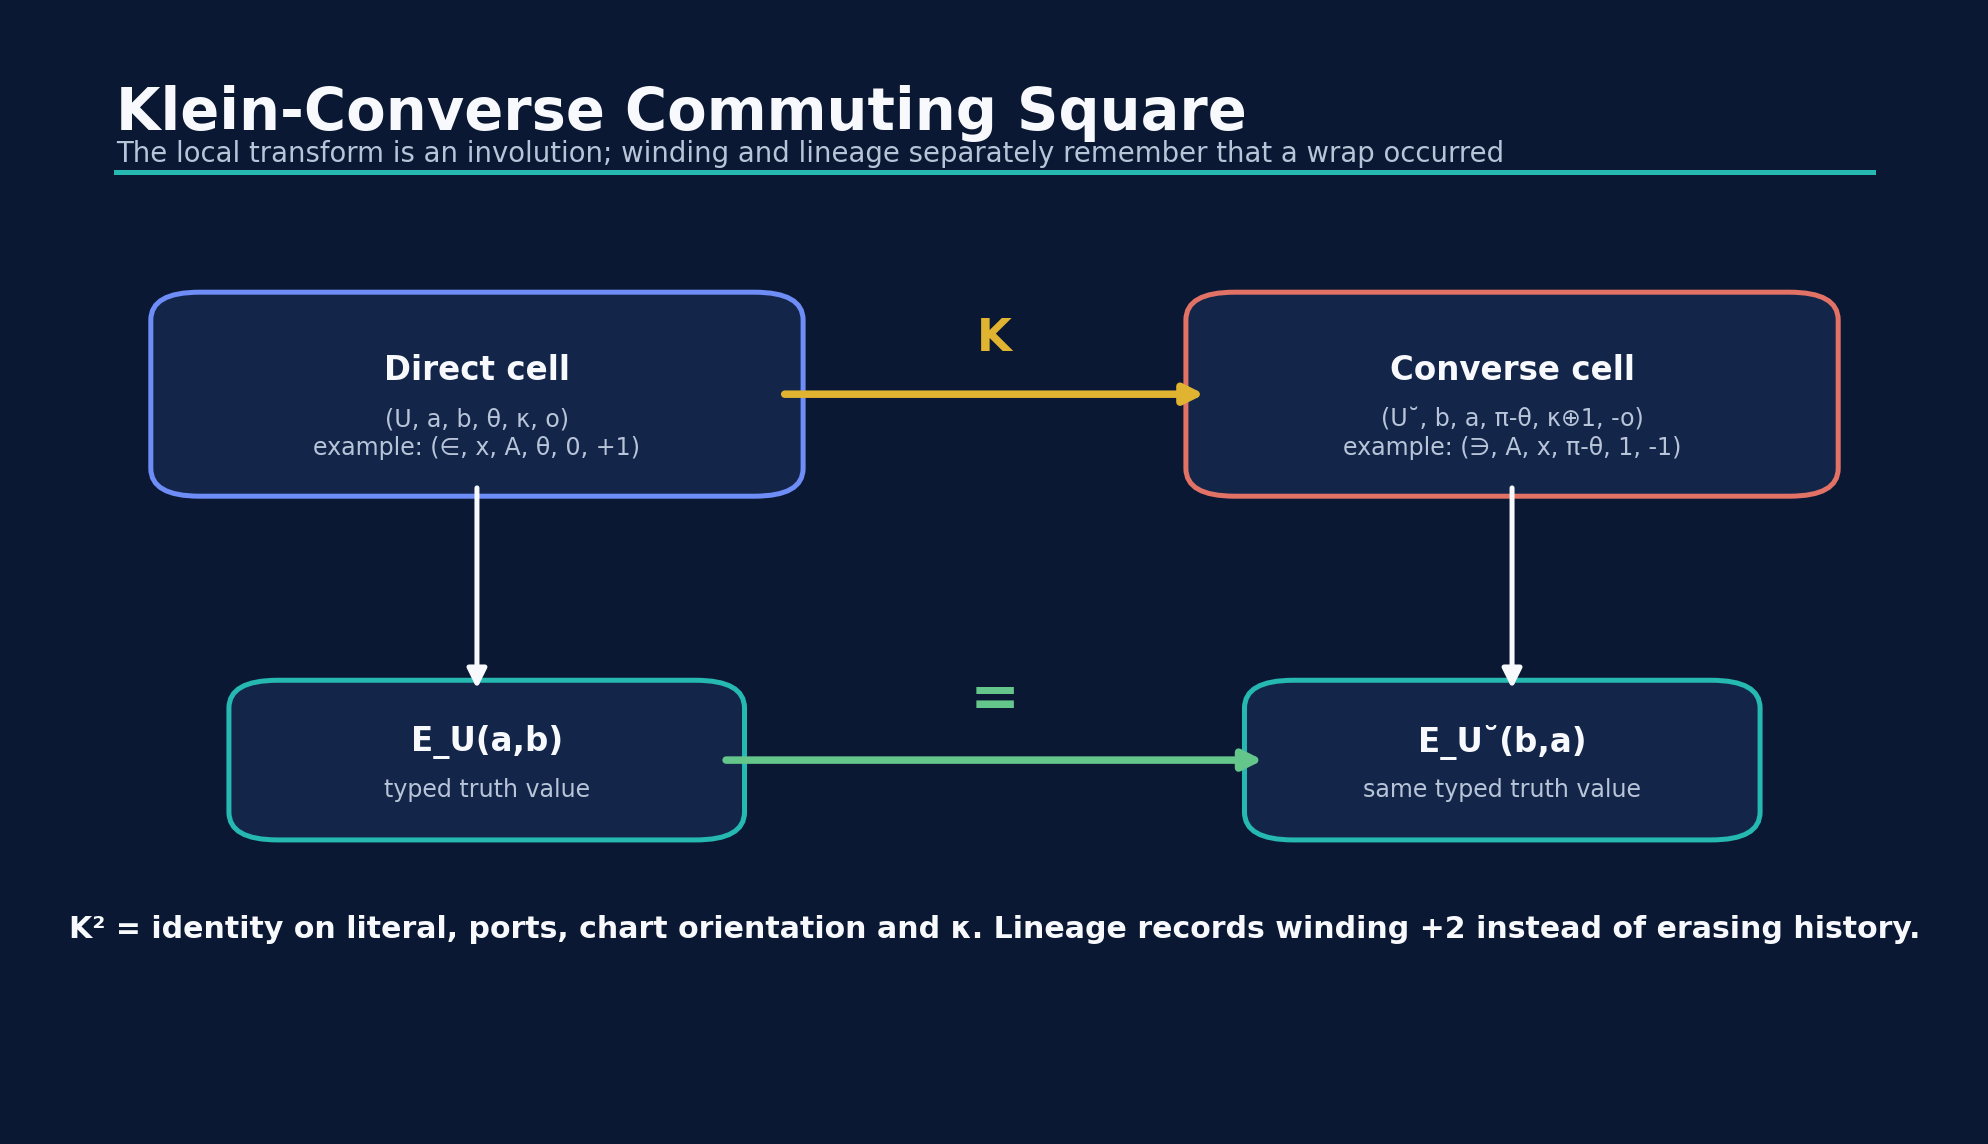
\includegraphics[width=0.94\textwidth]{klein_converse_square.png}
\caption{The semantic square commutes while lineage separately records the wrap.}
\end{figure}

\subsection{Reflective quotient}
A genuine reflective quotient requires a declared boundary identification such as
\[
(\rho_{\max},\theta,\kappa,o)
\sim
(\rho_{\min},\pi-\theta,\kappa\oplus1,-o).
\]
The angular derivative is \(-1\). That is the orientation-reversing feature. Merely adding \(\pi\) to \(\theta\) is a rotation and remains a different profile. \source{S3}

\subsection{Discrete angle maps}
For a 256-bin absolute angle code,
\[
q'=(128-q)\bmod 256.
\]
For a local delta code whose chart origin is transformed separately,
\[
\Delta q'=(-\Delta q)\bmod 256.
\]
Both maps are exact involutions in the finite code space.

\section{Canonical Glyph SDFs}
\subsection{Canonical profile}
The reference glyph profile is \texttt{ugts.canonical.capsule-glyph.v1}. A glyph is a finite segment skeleton \(S_U\) with stroke radius \(r_s\). Its field is
\[
G_U(p)=\min_{e\in S_U}d(p,e)-r_s.
\]
This is an exact Euclidean SDF to the finite union of equal-radius segment capsules that defines the canonical profile. The open ellipse is approximated by a fixed, versioned polyline; the exactness claim applies to that capsule union, not to an ideal analytic ellipse or to a third-party font.

\subsection{Mirror law}
For direct/converse relation pairs:
\[
G_{U^{\smile}}(x,y)=G_U(-x,y).
\]
The same reflection that changes visible port direction also matches the operand-converse map.

\begin{figure}[H]
\centering
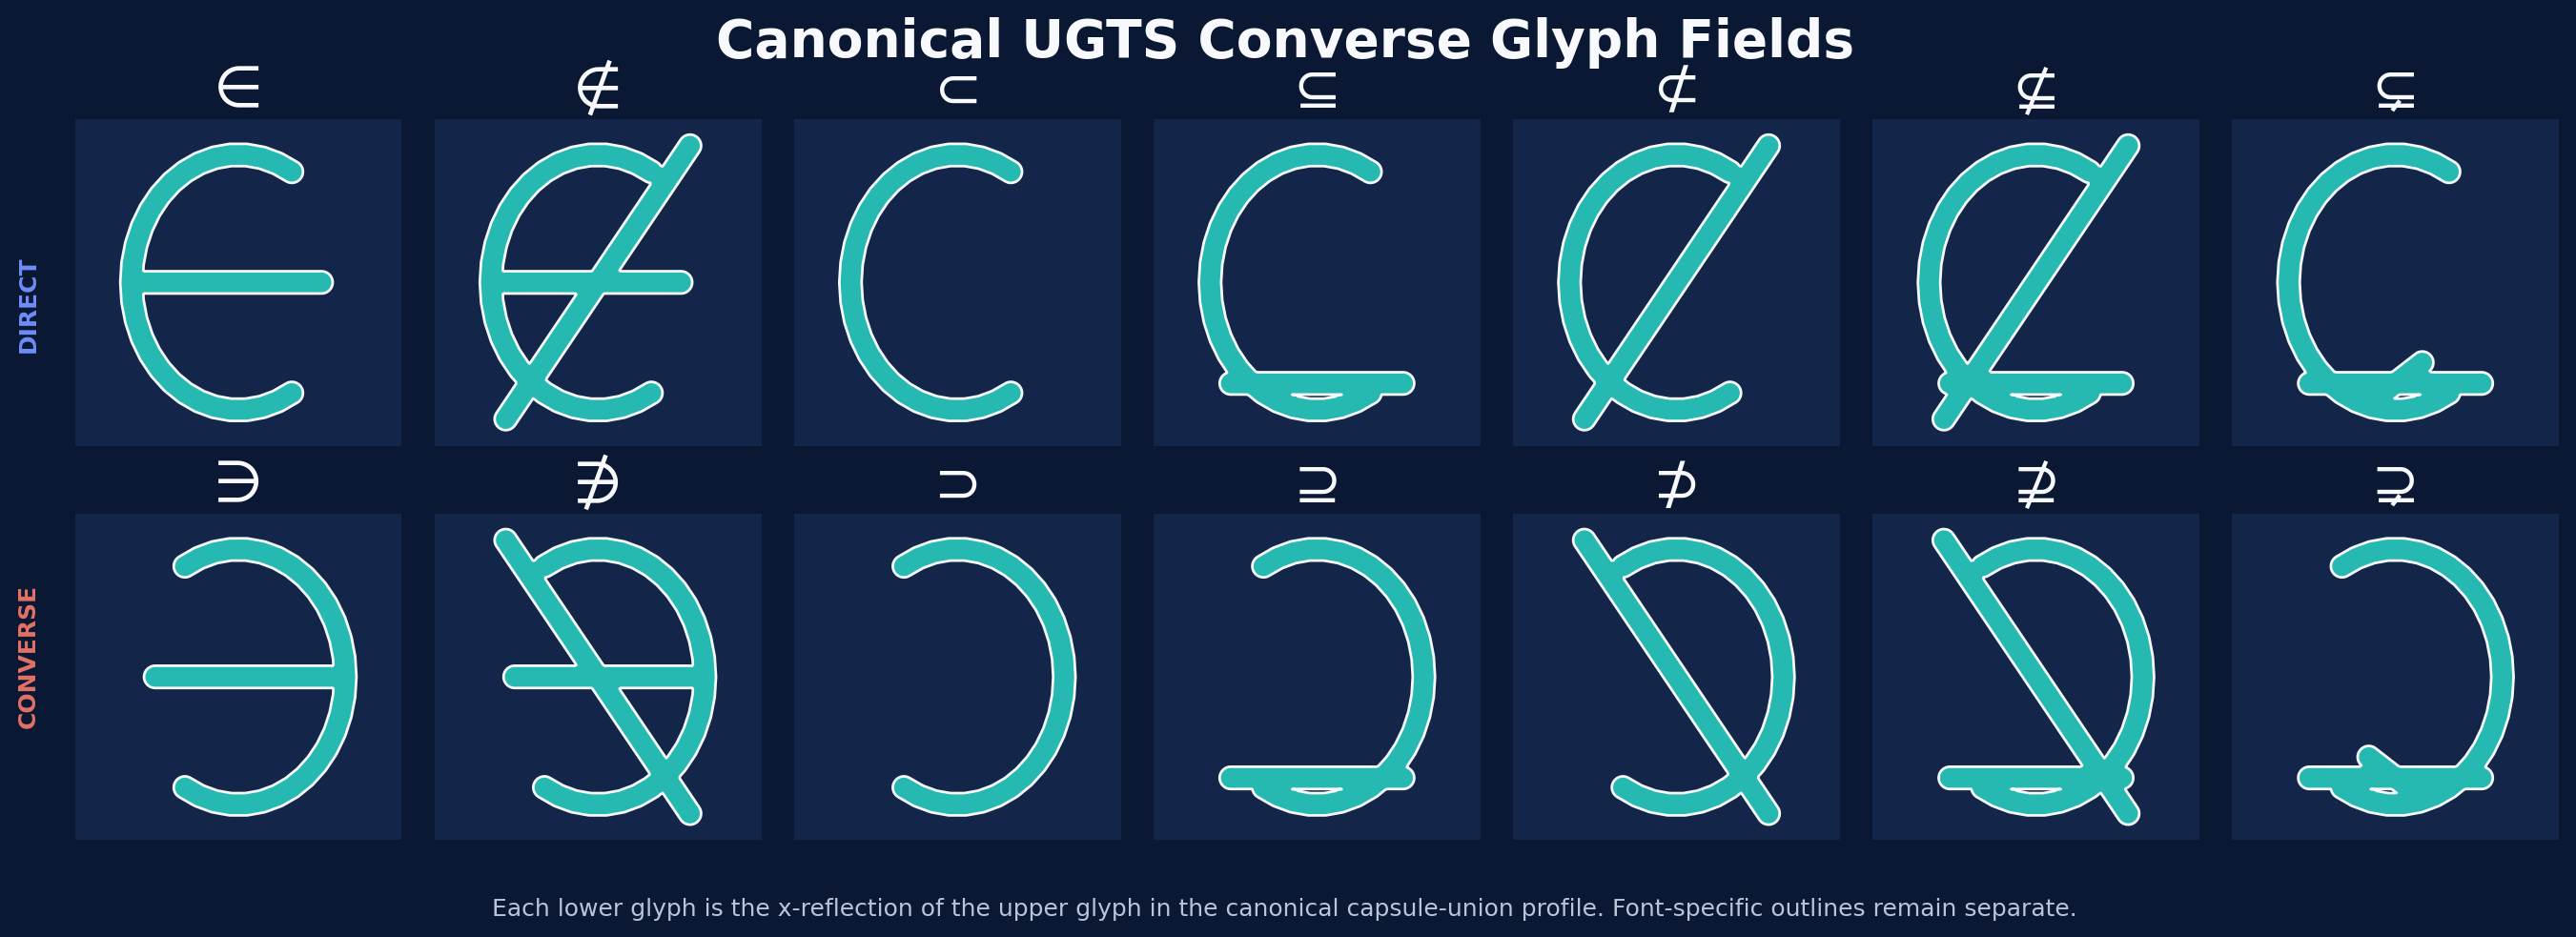
\includegraphics[width=\textwidth]{glyph_converse_plate.png}
\caption{Fourteen shipped converse glyph fields. The lower row is the exact x-reflection of the upper row in the canonical profile.}
\end{figure}

\subsection{Font-exact mode}
A font profile may provide measured or extracted outlines for each literal. In that mode, font, size, style, hinting, antialias threshold, fill/stroke and connectivity are part of the record. Semantic converse remains exact, while geometric mirror equality becomes profile-bound. This directly preserves BEA's boundary/equivalence separation. \source{S2}

\begin{boundarybox}
A Unicode codepoint fixes a character identity, not a unique visual outline. The canonical UGTS glyph is one deliberate, auditable geometry profile and never masquerades as every font.
\end{boundarybox}

\section{Cold Atlas, Hot Codebook and LUT}
\begin{figure}[H]
\centering
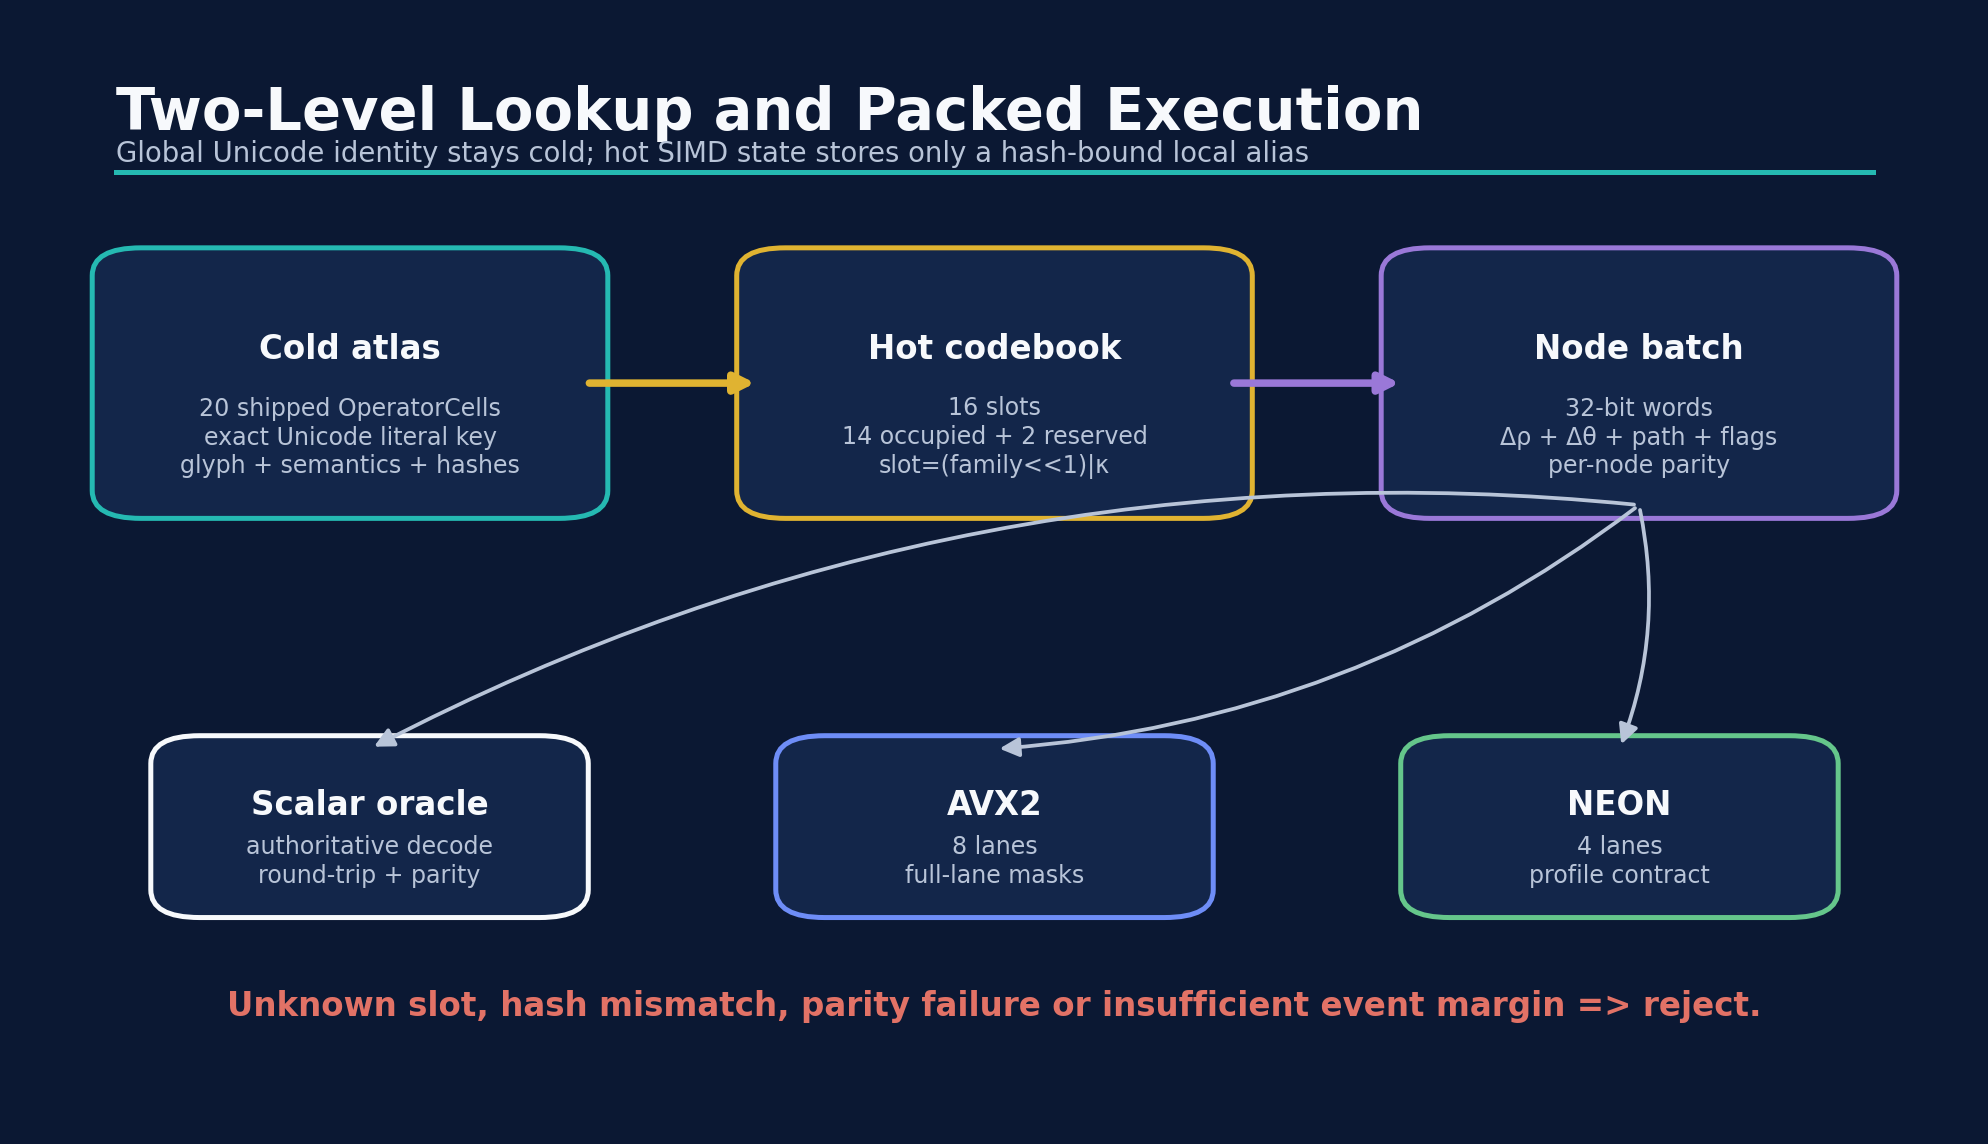
\includegraphics[width=0.98\textwidth]{atlas_codebook_packing.png}
\caption{The local opcode is a cache alias bound to the exact global atlas.}
\end{figure}

\subsection{Cold atlas}
The cold atlas is keyed by exact literal Unicode sequence and contains all 20 OperatorCells. Its 5.0 hash is:
\begin{Verbatim}[fontsize=\small,frame=single]
d4745a198469ff97665825f53d88cdbf8bad27687a3021c89177eedb83a55e91
\end{Verbatim}
It is the authority for Unicode identity, typed meaning, glyph profile, converse mapping and exactness metadata.

\subsection{Hot codebook}
The shipped \texttt{ugts.set-core-16.v1} codebook contains exactly 16 slots. Slots 0--13 map seven converse families; 14--15 are reserved and reject. Its hash is:
\begin{Verbatim}[fontsize=\small,frame=single]
3a279c68331d697f31e223b71eea898a4239d4da989b6f6d5c1dfd0dfcffb009
\end{Verbatim}

\rowcolors{2}{UGTSLight}{white}
\begin{longtable}{P{13mm}P{15mm}P{12mm}P{18mm}P{90mm}}
\toprule
\textbf{Slot} & \textbf{Family} & \textbf{\(\kappa\)} & \textbf{Literal} & \textbf{Operator ID}\\
\midrule
\endfirsthead
\toprule
\textbf{Slot} & \textbf{Family} & \textbf{\(\kappa\)} & \textbf{Literal} & \textbf{Operator ID}\\
\midrule
\endhead
\bottomrule
\endlastfoot
% BEGIN GENERATED codebook_table
0 & 0 & 0 & \(∈\) & set.membership.element-of \\
1 & 0 & 1 & \(∋\) & set.membership.contains-as-member \\
2 & 1 & 0 & \(∉\) & set.membership.not-element-of \\
3 & 1 & 1 & \(∌\) & set.membership.does-not-contain-as-member \\
4 & 2 & 0 & \(⊂\) & set.inclusion.proper-subset \\
5 & 2 & 1 & \(⊃\) & set.inclusion.proper-superset \\
6 & 3 & 0 & \(⊆\) & set.inclusion.subset-or-equal \\
7 & 3 & 1 & \(⊇\) & set.inclusion.superset-or-equal \\
8 & 4 & 0 & \(⊄\) & set.inclusion.not-proper-subset \\
9 & 4 & 1 & \(⊅\) & set.inclusion.not-proper-superset \\
10 & 5 & 0 & \(⊈\) & set.inclusion.not-subset-or-equal \\
11 & 5 & 1 & \(⊉\) & set.inclusion.not-superset-or-equal \\
12 & 6 & 0 & \(⊊\) & set.inclusion.subset-with-not-equal \\
13 & 6 & 1 & \(⊋\) & set.inclusion.superset-with-not-equal \\
14 & - & - & reserved & - \\
15 & - & - & reserved & - \\
% END GENERATED codebook_table
\end{longtable}

\subsection{Literal-to-LUT path}
A lookup proceeds as follows:
\begin{enumerate}
\item Normalize and resolve the exact Unicode literal in the cold atlas.
\item Verify the cell hash and atlas hash.
\item Select or build a hot codebook whose entries commit to those hashes.
\item Store only the local four-bit slot in packed nodes.
\item Decode the slot through the codebook before semantic or glyph evaluation.
\end{enumerate}
Unknown code, codebook mismatch or atlas mismatch is a hard failure.

\section{Packed Log-Polar Node 32}
\begin{figure}[H]
\centering
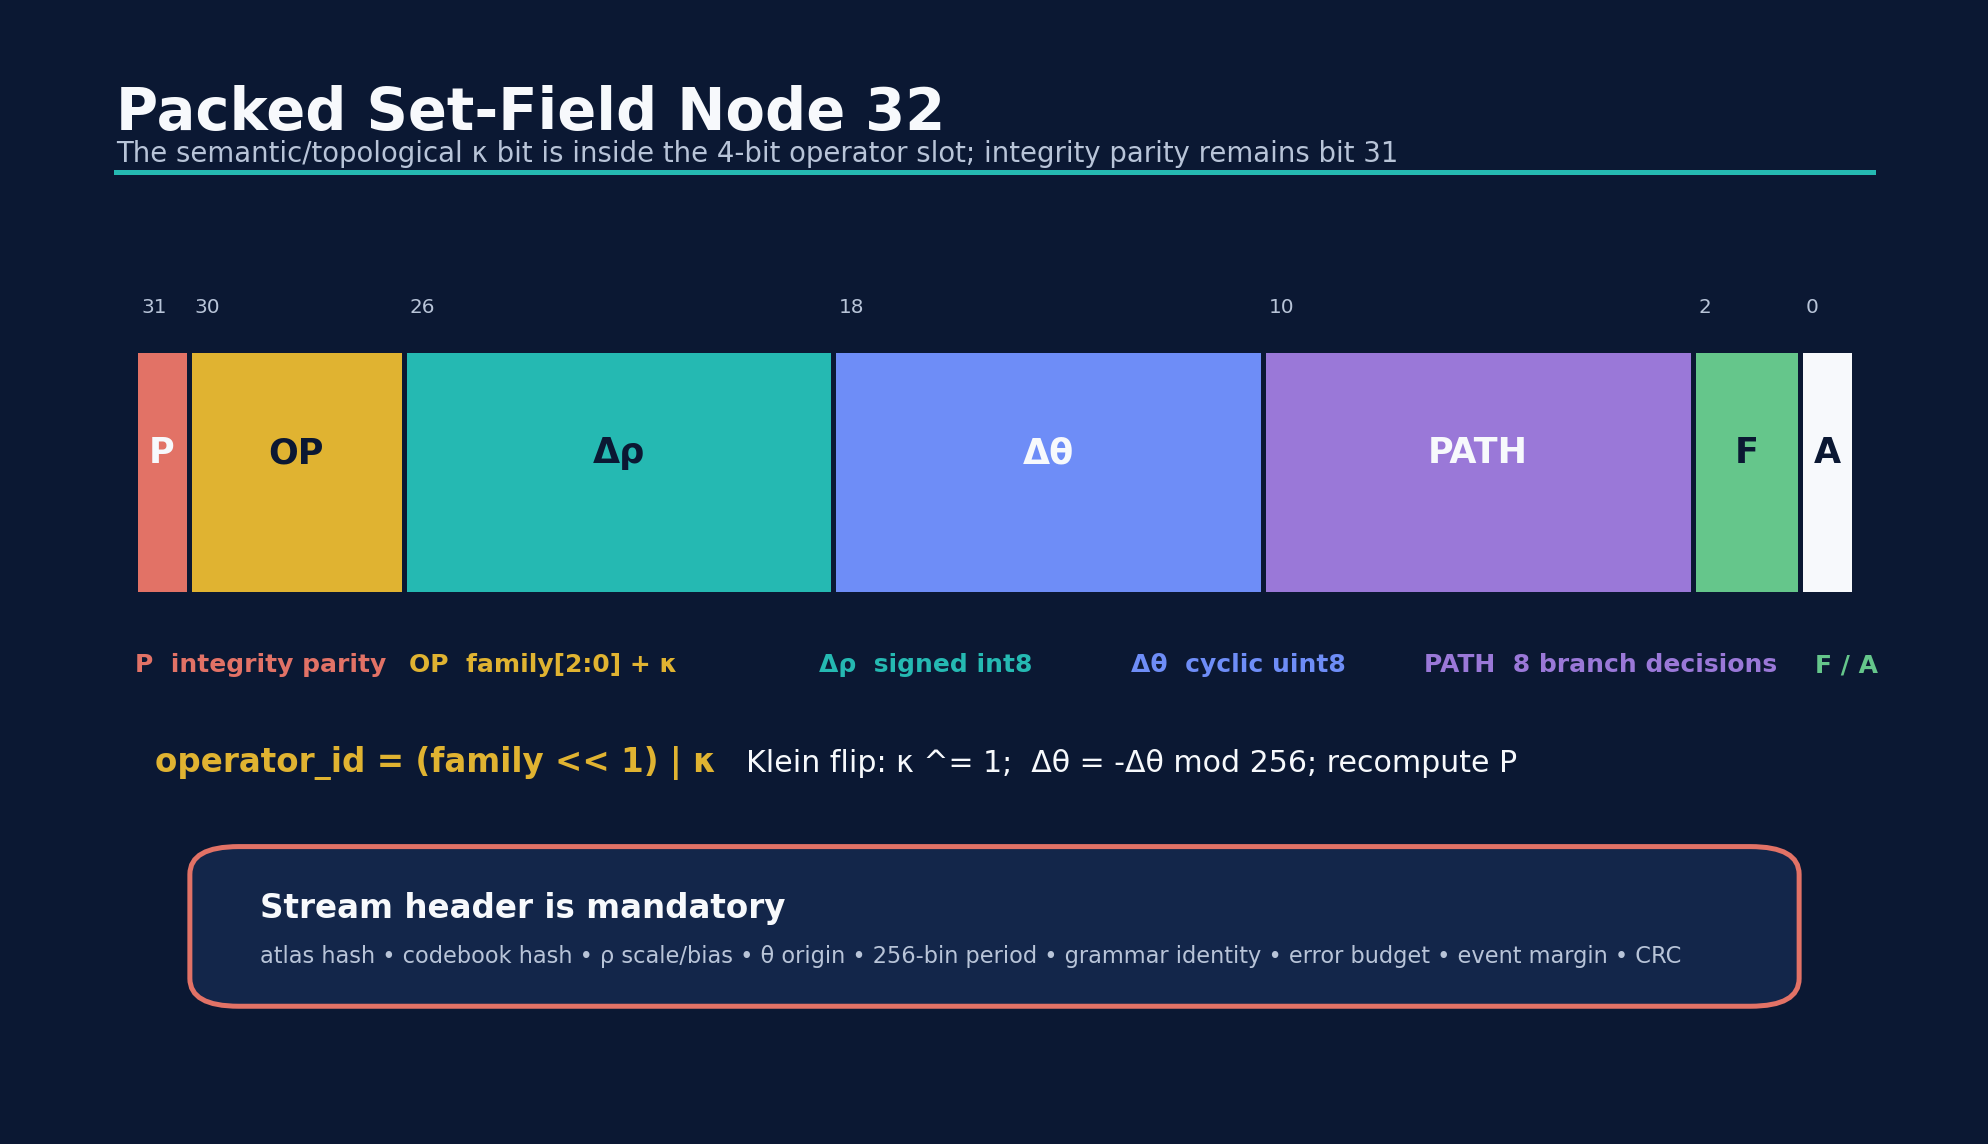
\includegraphics[width=\textwidth]{packed_node_layout.png}
\caption{Corrected bit layout with separate integrity and topological roles.}
\end{figure}

\subsection{Bit layout}
\begin{tabularx}{\textwidth}{P{22mm}P{25mm}P{30mm}Y}
\toprule
\textbf{Bits} & \textbf{Width} & \textbf{Field} & \textbf{Contract}\\
\midrule
31 & 1 & integrity parity & parity of payload bits 0--30; not \(\kappa\)\\
30--27 & 4 & operator slot & three-bit family plus one-bit \(\kappa\)\\
26--19 & 8 & \(\Delta\rho\) & signed int8; scale/bias supplied by header\\
18--11 & 8 & \(\Delta\theta\) & cyclic uint8; 256-bin period\\
10--3 & 8 & grammar path & bounded eight-decision branch fragment\\
2--1 & 2 & local flags & profile-defined status; narrow meanings only\\
0 & 1 & active & explicitly decoded and tested\\
\bottomrule
\end{tabularx}

\subsection{Packing formula}
Let \(s=(f,\kappa,\Delta\rho,\Delta\theta,p,g,a)\). The payload is
\[
\begin{split}
\mathrm{payload}={}&((2f+\kappa)\ll27)
\;|\;((\Delta\rho\bmod256)\ll19)\\
&|\;(\Delta\theta\ll11)
\;|\;(p\ll3)
\;|\;(g\ll1)
\;|\;a.
\end{split}
\]
Bit 31 equals the population parity of bits 0--30, giving even parity over the full word.

\subsection{Two parities, two roles}
\begin{itemize}
\item \(\kappa\) is the semantic/topological direct-versus-converse selector.
\item bit 31 is an integrity precheck.
\end{itemize}
A legitimate \(\texttt{∈}\to\texttt{∋}\) transition toggles \(\kappa\), then recomputes the integrity parity. The two roles can never share one bit.

\subsection{Mandatory stream header}
The 32-bit word is not self-describing. The stream header carries:
\begin{itemize}
\item schema, atlas and codebook IDs and hashes;
\item \(\rho\) origin, scale, bias and admissible range;
\item \(\theta\) origin, period and rounding rule;
\item reflective wrap profile;
\item grammar definition and path-prefix context;
\item capability and exactness policy;
\item error budget and event-margin rule;
\item block CRC and optional outer content hash.
\end{itemize}

The reference \texttt{UG5N} framing uses a canonical JSON header, little-endian 32-bit words and CRC32 over prefix, header and node payload.

\subsection{Quantization}
A full circle with 256 bins has bin width
\[
\frac{360^{\circ}}{256}=1.40625^{\circ}.
\]
With round-to-nearest, maximum half-bin angular error is
\[
0.703125^{\circ}.
\]
Radial error depends on the declared \(\Delta\rho\) scale. Packed evaluation may be promoted only when total numeric error remains below the relevant event margin.

\subsection{Bounded grammar path}
Eight path bits encode eight binary decisions or one fragment of a longer externally stored address. They do not encode an unbounded tree, infinite detail or a complete world.

\section{Scalar and SIMD Execution Profiles}
\subsection{Scalar oracle}
The dependency-free Python and C++20 scalar codecs are the conformance authority. Every backend must match:
\begin{itemize}
\item field extraction and signed \(\Delta\rho\) decoding;
\item active and local flags;
\item operator family and \(\kappa\);
\item parity verification;
\item Klein flip and round trip;
\item codebook resolution;
\item error and capability status.
\end{itemize}

\subsection{AVX2 eight-lane extraction}
The optional header \texttt{native/ugts5\_avx2.hpp} loads eight words and extracts fields with shifts and masks. It corrects two common source errors:
\begin{enumerate}
\item reading bit 31 is not parity verification; a tested popcount/XOR fold or scalar check is still required;
\item a 0/1 selector must be expanded to \texttt{0x00000000}/\texttt{0xffffffff} before lane-wise selection.
\end{enumerate}

The reference mask expansion is conceptually
\[
M=0-\kappa,
\]
so each 32-bit lane becomes all-zero or all-one.

\subsection{ARM NEON profile}
The NEON contract mirrors the AVX2 layout in four lanes and uses full-lane masks before \texttt{vbslq\_u32}. It is specified but not measured in this package.

\subsection{Branch strategy}
Evaluate-both-and-select can help when both branches are cheap and coherence is poor. It can waste work when either branch is expensive. A backend may choose among scalar branching, active-lane compaction, dual evaluation or measured automatic selection. No universal speed claim is promoted.

\subsection{Benchmark boundary}
Cycle counts, cache residency, SIMD utilization, latency and energy require a named processor, compiler flags, workload, precision, equal-error baseline and captured measurement. The package proves codec conformance, not target performance. \source{S4}

\section{Exactness, Proof and Certification}
\subsection{Point query versus global relation}
A point membership query can be a local field comparison. Subset, equality and emptiness are global relations:
\[
A\subseteq B\iff\forall x\in X:\ x\in A\Rightarrow x\in B.
\]
No packed local lookup turns the quantifier into universal constant-time proof.

\subsection{Certificate object}
A version-5 relation certificate contains:
\[
C=(U,h_U,\mathrm{profile},\mathrm{operands},\mathrm{scope},\mathrm{capability},I,e,m,r,N),
\]
where \(I\) is the result or interval, \(e\) numeric error, \(m\) event margin, \(r\) reason/status and \(N\) explicit non-claims.

\subsection{Finite exact proof}
For a declared finite universe, the runtime can exhaustively check membership, subset, proper subset, equality and emptiness. The universe ordering is part of the proof input. Changing the universe invalidates the certificate.

\subsection{Continuous proof}
A continuous-domain claim requires at least one of:
\begin{itemize}
\item an analytic proof;
\item interval arithmetic covering the full domain;
\item a certified spatial subdivision with a proven residual bound;
\item a theorem-specific decision procedure;
\item another explicitly verified completeness argument.
\end{itemize}
A sampled LUT remains sampled evidence unless the certificate closes the between-sample gap.

\subsection{Integrity ladder}
\begin{tabularx}{\textwidth}{P{38mm}Y}
\toprule
\textbf{Layer} & \textbf{Role}\\
\midrule
Per-node parity & fast odd-bit corruption precheck\\
Stream CRC32 & accidental block corruption detection\\
Operator-cell hash & content identity of one definition\\
Atlas/codebook hash & exact lookup-context binding\\
Pre/post state hash & authoritative transition identity\\
Lineage/replay & ordered explanation of how state was reached\\
\bottomrule
\end{tabularx}
No single layer substitutes for the others.

\section{Integration with UGTS State Authority}
\subsection{Pure evaluation is upstream}
A Unicode cell may answer a set relation, return a glyph field value, transform a signed set field, select a converse, decode a packed node or issue an exactness certificate. None of those operations changes authoritative world state by itself.

\subsection{Canonical handoff}
A state-changing application uses:
\begin{Verbatim}[fontsize=\small,frame=single]
operator result + support evidence
 -> compatibility
 -> guard / error / uncertainty
 -> verified proposal
 -> deterministic conflict resolution
 -> atomic commit
 -> pre/post hashes
 -> lineage + replay
 -> optional glyph, display, storage or device projection
\end{Verbatim}

\subsection{Example: membership-triggered transition}
Suppose a rule proposes opening a gate when token \(x\) belongs to set \(A\). The OperatorCell answers \(x\in A\). The application must still prove that the rule is supported at this gate, the token and gate are compatible, timing and uncertainty guards pass, and the resulting patch preserves required invariants. Only then is the gate state committed.

\subsection{Example: reflective route transition}
A route crossing a declared radial boundary may apply \(\mathcal{K}\). The local operator and orientation flip, but the transition is committed only after the boundary guard and topology profile verify. Winding and the selected quotient remain in lineage so repeated arrivals at the same coordinates are distinguishable.

\section{Reference Implementation and Validation}
\subsection{Package map}
\begin{tabularx}{\textwidth}{P{34mm}Y}
\toprule
\textbf{Path} & \textbf{Contents}\\
\midrule
\texttt{report/} & PDF report and editable XeLaTeX source\\
\texttt{src/ugts5/} & canonical hashing, atlas, set fields, glyph SDF, Klein transform, packing, stream and CLI\\
\texttt{spec/} & schemas, atlas, codebook, release record, source register, mechanisms and claims\\
\texttt{native/} & C++20 scalar codec, AVX2 extraction header and NEON contract\\
\texttt{examples/} & operator, field and packed-stream demonstrations\\
\texttt{tests/} & 83 standard-library Python conformance tests\\
\texttt{validation/} & captured outputs, schema results, native results, hashes and manifests\\
\texttt{figures/} & report diagrams and glyph-field plate\\
\texttt{dist/} & built Python wheel\\
\bottomrule
\end{tabularx}

\subsection{Validation result}
\begin{figure}[H]
\centering
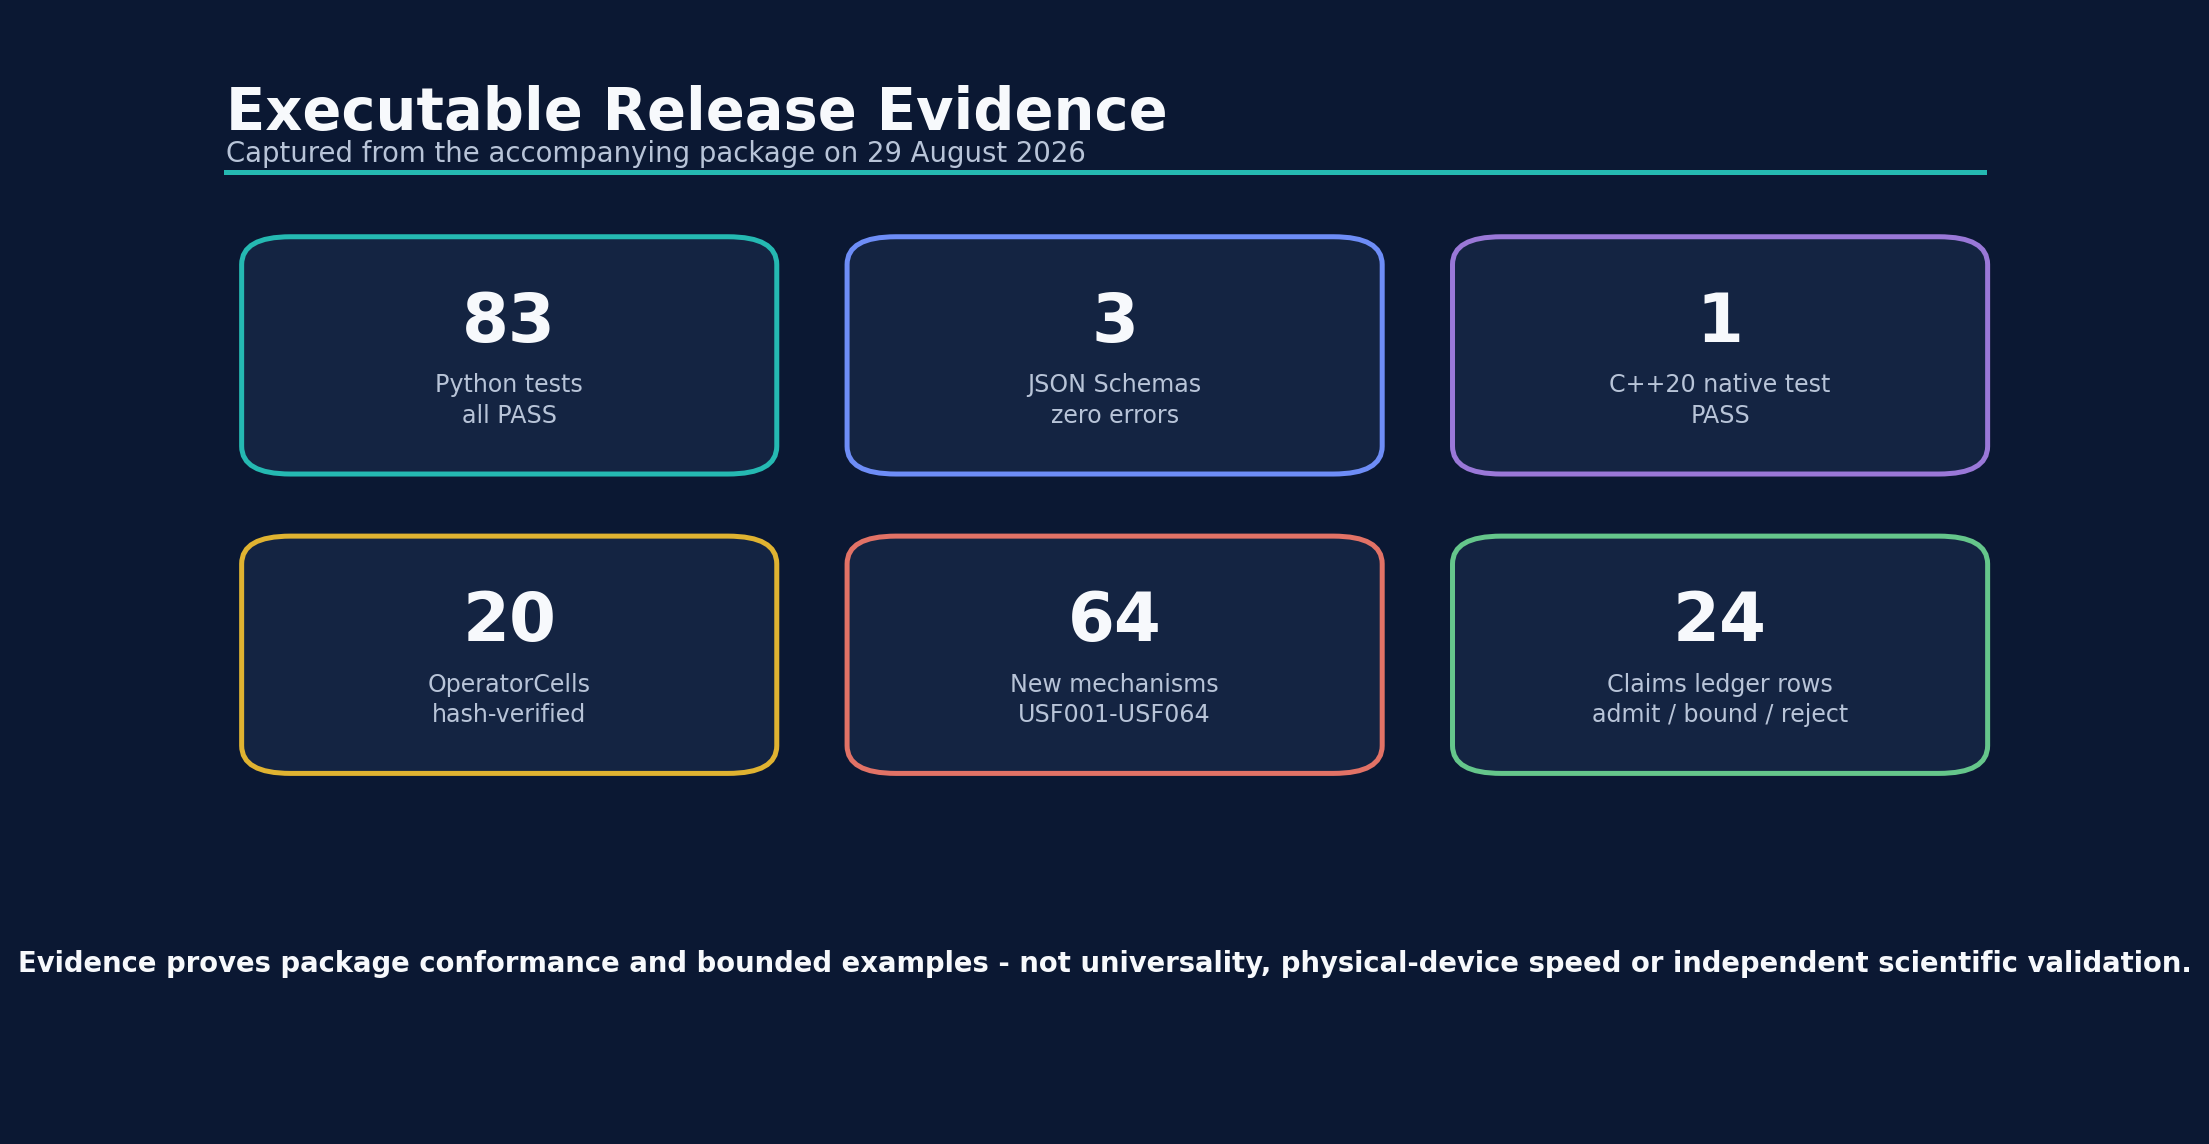
\includegraphics[width=0.98\textwidth]{validation_summary.png}
\caption{Exact captured package evidence.}
\end{figure}

\rowcolors{2}{UGTSLight}{white}
\begin{tabularx}{\textwidth}{P{48mm}P{42mm}Y}
\toprule
\textbf{Check} & \textbf{Scope} & \textbf{Result}\\
\midrule
% BEGIN GENERATED validation_table
Python conformance & 83 tests & PASS \\
JSON Schema & 3 instances & 0 errors \\
Native scalar codec & C++20 & PASS \\
Operator atlas & 20 cells & all content hashes verified \\
Hot codebook & 16 slots & 14 assigned / 2 reserved \\
Mechanism delta & 64 rows & USF001-USF064 / M886-M949 \\
Claims ledger & 24 rows & admit / bound / reject recorded \\
Wheel & py3-none-any & built and clean-installed \\
% END GENERATED validation_table
\bottomrule
\end{tabularx}

\subsection{What the tests establish}
The tests establish deterministic canonical JSON, content-hash verification, Unicode scalar/UTF-8 round trip, signed-field truth tables, finite exact set relations, glyph reflection, local Klein involution, discrete angle involution, packed round trip, active-bit decoding, integrity parity behavior, stream CRC, codebook rejection, schema validity and native scalar parity with the Python layout.

\subsection{What the tests do not establish}
The tests are not independent scientific validation. They do not prove every font mirrors converse glyphs, every set has a metric SDF, continuous subset claims are solved, AVX2 or NEON are faster, physical hardware is low-power, or the formalism is complete for all Unicode mathematics.

\subsection{Reproduction}
\begin{Verbatim}[fontsize=\small,frame=single]
python tools/generate_specs.py
python examples/packed_stream_demo.py
python -m unittest discover -s tests -v
python tools/validate_schemas.py
c++ -std=c++20 -O2 -I native native/test_packed_node.cpp -o /tmp/ugts5_native
/tmp/ugts5_native
python -m ugts5 verify --package-root .
\end{Verbatim}

\section{Claims Ledger Summary}
The complete 24-row ledger is in Appendix D and in \texttt{spec/claims\_ledger.json/csv}. The governing decisions are:

\begin{tabularx}{\textwidth}{P{50mm}P{31mm}Y}
\toprule
\textbf{Claim} & \textbf{Disposition} & \textbf{Reason}\\
\midrule
Unicode can address shape and functionality & ADMIT & One typed cell co-addresses literal, glyph, evaluator and field action.\\
Geometry and semantics are identical & REJECT & They remain distinct domains connected by explicit maps.\\
Set theory can use signed set fields & ADMIT WITH CAPABILITY & Exact SDF is one class; finite, metric, residual and oracle fields remain distinct.\\
Converse pairs share a semantic kernel & ADMIT & Typed port normalization makes the reuse exact.\\
Klein flip is just a bit shift & CORRECT & It selects an involution that swaps operands and reflects the chart.\\
One bit can be integrity and topology & REJECT & \(\kappa\) and parity are separate fields.\\
Four-bit operator ID is global & REJECT & It is a hash-bound local codebook alias.\\
Packed node is complete state & REJECT & Definitions, header, uncertainty, lineage and hashes remain external.\\
Composed fields remain exact SDFs & REJECT & Sign is preserved; exact distance may be lost.\\
SIMD is automatically faster & REJECT & A named target and equal-error benchmark are required.\\
Deterministic parity is true randomness & REJECT & Determinism supplies repeatability, not entropy.\\
This atlas enumerates all mathematics & REJECT & The shipped atlas is bounded and the schema is extensible.\\
\bottomrule
\end{tabularx}

\section{Acceptance, Kill Criteria and Final Definition}
\subsection{Acceptance gates}
A version-5 use is accepted only when:
\begin{enumerate}
\item the exact Unicode scalar sequence resolves;
\item the OperatorCell and atlas hashes verify;
\item the operand types and surface-to-canonical port map validate;
\item the field capability is no stronger than the evidence;
\item the converse and glyph profile are declared;
\item the codebook and stream header match;
\item per-node parity and stream CRC pass;
\item quantization error stays below the declared event margin;
\item state mutation proceeds through the canonical authority chain;
\item lineage records accepted transitions and relevant wraps.
\end{enumerate}

\subsection{Kill criteria}
Reject or narrow the use when:
\begin{itemize}
\item Unicode identity is replaced by an undocumented local opcode;
\item font geometry is treated as profile-free;
\item semantic zero is called glyph-SDF zero;
\item a sampled LUT is presented as a continuous-domain proof;
\item \(\kappa\) is overloaded as integrity, randomness, uncertainty or complete state;
\item a half-turn is mislabeled as reflective Klein gluing;
\item an unknown codebook slot aliases an existing operator;
\item min/max field composition silently retains exact-SDF status;
\item backend output differs from the scalar oracle;
\item performance or compression claims omit a named target, workload and equal-error baseline;
\item operator evaluation bypasses support, compatibility, guard, commit or lineage.
\end{itemize}

\subsection{Final upgraded definition}
\begin{definitionbox}
UGTS Foundation 5.0 is a literal, content-addressed Unicode operator substrate in which set relations and set algebra may be evaluated through typed signed set fields; canonical glyph shapes are executable SDF definitions; converse surface spellings share canonical semantic kernels; reflective Klein transitions reverse typed ports, glyph orientation and chart orientation through an explicit involution; and compact log-polar execution records remain hash-bound, error-bounded and downstream of authoritative definitions.
\end{definitionbox}

\begin{conclusionbox}
A Unicode operator is no longer merely text and no longer merely an icon. It is a content-addressed, executable geometric rule cell whose literal codepoint resolves both its canonical shape and its typed operation. A Klein-converse parity flip mirrors the shape, reverses the typed ports and selects the converse Unicode spelling while preserving the mathematical truth value.
\end{conclusionbox}

\begin{evidencebox}
The word \emph{parity} in the conclusion names the direct/converse \(\kappa\) selector as a two-state orientation parity. It does not merge with bit-31 integrity parity, random entropy, uncertainty, identity or full state. The package and schemas keep those roles separate.
\end{evidencebox}

\clearpage
\appendix
\section{Complete Shipped Unicode Operator Atlas}
\small
\rowcolors{2}{UGTSLight}{white}
\begin{longtable}{P{7mm}P{18mm}P{10mm}P{10mm}P{10mm}P{27mm}P{65mm}}
\toprule
\textbf{Lit.} & \textbf{Scalar} & \textbf{Fam.} & \textbf{\(\kappa\)} & \textbf{Conv.} & \textbf{Kernel} & \textbf{Stable operator ID}\\
\midrule
\endfirsthead
\toprule
\textbf{Lit.} & \textbf{Scalar} & \textbf{Fam.} & \textbf{\(\kappa\)} & \textbf{Conv.} & \textbf{Kernel} & \textbf{Stable operator ID}\\
\midrule
\endhead
\bottomrule
\endlastfoot
% BEGIN GENERATED operator_table
\(∈\) & U+2208 & 0 & 0 & \(∋\) & membership & set.membership.element-of \\
\(∋\) & U+220B & 0 & 1 & \(∈\) & membership & set.membership.contains-as-member \\
\(∉\) & U+2209 & 1 & 0 & \(∌\) & nonmembership & set.membership.not-element-of \\
\(∌\) & U+220C & 1 & 1 & \(∉\) & nonmembership & set.membership.does-not-contain-as-member \\
\(⊂\) & U+2282 & 2 & 0 & \(⊃\) & proper subset & set.inclusion.proper-subset \\
\(⊃\) & U+2283 & 2 & 1 & \(⊂\) & proper subset & set.inclusion.proper-superset \\
\(⊆\) & U+2286 & 3 & 0 & \(⊇\) & subset or equal & set.inclusion.subset-or-equal \\
\(⊇\) & U+2287 & 3 & 1 & \(⊆\) & subset or equal & set.inclusion.superset-or-equal \\
\(⊄\) & U+2284 & 4 & 0 & \(⊅\) & not proper subset & set.inclusion.not-proper-subset \\
\(⊅\) & U+2285 & 4 & 1 & \(⊄\) & not proper subset & set.inclusion.not-proper-superset \\
\(⊈\) & U+2288 & 5 & 0 & \(⊉\) & not subset or equal & set.inclusion.not-subset-or-equal \\
\(⊉\) & U+2289 & 5 & 1 & \(⊈\) & not subset or equal & set.inclusion.not-superset-or-equal \\
\(⊊\) & U+228A & 6 & 0 & \(⊋\) & proper subset variant & set.inclusion.subset-with-not-equal \\
\(⊋\) & U+228B & 6 & 1 & \(⊊\) & proper subset variant & set.inclusion.superset-with-not-equal \\
\(∪\) & U+222A & - & - & - & union & set.algebra.union \\
\(∩\) & U+2229 & - & - & - & intersection & set.algebra.intersection \\
\(∖\) & U+2216 & - & - & - & difference & set.algebra.difference \\
\(∁\) & U+2201 & - & - & - & complement & set.algebra.complement \\
\(∅\) & U+2205 & - & - & - & empty set & set.literal.empty \\
\(=\) & U+003D & - & - & - & set equality & set.relation.equality \\
% END GENERATED operator_table
\end{longtable}
\normalsize

\section{Hot Codebook Set-Core-16}
The table in Section 9 is normative. Slots 14 and 15 are reserved and must reject unless a different versioned codebook is selected in the stream header. The four-bit value is never globally meaningful without the codebook hash.

\section{Complete Mechanism Delta USF001--USF064}
\scriptsize
\rowcolors{2}{UGTSLight}{white}
\begin{longtable}{P{20mm}P{15mm}P{28mm}P{70mm}P{20mm}}
\toprule
\textbf{ID} & \textbf{Domain} & \textbf{Name} & \textbf{Definition} & \textbf{Validation}\\
\midrule
\endfirsthead
\toprule
\textbf{ID} & \textbf{Domain} & \textbf{Name} & \textbf{Definition} & \textbf{Validation}\\
\midrule
\endhead
\bottomrule
\endlastfoot
% BEGIN GENERATED mechanism_table
USF001 / M886 & release & Release identity & Component-scoped major release identity with legacy UGTS-KC 5.0 alias. & implemented-and-tested \\
USF002 / M887 & source & Source register & Content-hashed source and parent register without raw-source redistribution. & implemented-and-tested \\
USF003 / M888 & referential & OperatorCell & One content-addressed record co-addresses literal, glyph, semantics and field action. & implemented-and-tested \\
USF004 / M889 & unicode & Unicode scalar key & Exact Unicode scalar sequence is a canonical cold-atlas lookup key. & implemented-and-tested \\
USF005 / M890 & unicode & UTF-8 literal key & UTF-8 spelling is recorded and round-tripped without ASCII aliasing. & implemented-and-tested \\
USF006 / M891 & unicode & NFC normalization profile & NFC is explicit; compatibility normalization is not silently applied. & implemented-and-tested \\
USF007 / M892 & typing & Typed signature & Every operator declares domain, codomain, arity and type parameters. & implemented-and-tested \\
USF008 / M893 & typing & Canonical argument order & One semantic port order is authoritative for each converse family. & implemented-and-tested \\
USF009 / M894 & typing & Surface argument map & Surface operands map explicitly to canonical semantic ports. & implemented-and-tested \\
USF010 / M895 & semantics & Semantic evaluator & Literal dispatch selects a bounded typed semantic kernel. & implemented-and-tested \\
USF011 / M896 & geometry & Canonical glyph SDF & A versioned capsule-union field represents the literal operator shape. & implemented-and-tested \\
USF012 / M897 & field & Set-field action & Operator records declare predicates or sign-compatible field transforms. & implemented-and-tested \\
USF013 / M898 & relation & Converse link & Direct and converse cells reference each other by stable operator ID. & implemented-and-tested \\
USF014 / M899 & integrity & Operator content hash & Every cell carries a canonical SHA-256 content address. & implemented-and-tested \\
USF015 / M900 & provenance & Provenance class & Source motif, engineering normalization and measured evidence stay distinct. & implemented-and-tested \\
USF016 / M901 & exactness & Capability class & Exact SDF, metric field, bound, residual, membership field and oracle remain distinct. & implemented-and-tested \\
USF017 / M902 & field & Signed set field & phi\_A = d(x,A) - d(x,X\textbackslash{}A) under a declared metric profile. & implemented-and-tested \\
USF018 / M903 & field & Characteristic fallback & Finite or non-metric sets can use a signed membership field. & implemented-and-tested \\
USF019 / M904 & relation & Membership predicate & x in A iff phi\_A(x) \textless{}= 0 under the selected boundary policy. & implemented-and-tested \\
USF020 / M905 & relation & Nonmembership predicate & x notin A is the typed negation of membership. & implemented-and-tested \\
USF021 / M906 & relation & Subset predicate & A subseteq B is a quantified emptiness claim over A\textbackslash{}B. & implemented-and-tested \\
USF022 / M907 & relation & Proper subset predicate & Proper inclusion adds non-equality to subset. & implemented-and-tested \\
USF023 / M908 & relation & Set equality & A=B is mutual inclusion under a common universe/profile. & implemented-and-tested \\
USF024 / M909 & relation & Empty-set predicate & Emptiness is exact only when the domain proof is complete. & implemented-and-tested \\
USF025 / M910 & field & Union field & min(phi\_A,phi\_B) preserves the union sign. & implemented-and-tested \\
USF026 / M911 & field & Intersection field & max(phi\_A,phi\_B) preserves the intersection sign. & implemented-and-tested \\
USF027 / M912 & field & Complement field & -phi\_A reverses inside and outside. & implemented-and-tested \\
USF028 / M913 & field & Difference field & max(phi\_A,-phi\_B) preserves the sign of A\textbackslash{}B. & implemented-and-tested \\
USF029 / M914 & field & Symmetric-difference field & A sign-correct max/min formula represents A triangle B. & implemented-and-tested \\
USF030 / M915 & exactness & Field capability downgrade & Composed fields never inherit exact-distance status without proof. & implemented-and-tested \\
USF031 / M916 & proof & Finite-universe proof & Exhaustive finite checks may issue exact relation certificates. & implemented-and-tested \\
USF032 / M917 & proof & Interval/analytic proof & Continuous global claims require analytic, interval or certified-cover evidence. & implemented-and-tested \\
USF033 / M918 & proof & Sample-only nonproof & A sampled LUT result is bounded evidence, not universal inclusion proof. & implemented-and-tested \\
USF034 / M919 & topology & Klein-converse transform & One transform reflects chart, swaps ports and toggles converse state. & implemented-and-tested \\
USF035 / M920 & topology & Operator converse & U maps to U-smile while preserving truth after operand exchange. & implemented-and-tested \\
USF036 / M921 & topology & Operand swap & Typed endpoints reverse rather than being reinterpreted in place. & implemented-and-tested \\
USF037 / M922 & geometry & Glyph reflection & Canonical converse glyph is the x-reflection of the direct glyph. & implemented-and-tested \\
USF038 / M923 & topology & Angular reflection & theta maps to pi-theta on the reflective profile. & implemented-and-tested \\
USF039 / M924 & topology & Orientation selector & kappa is a semantic/topological selector and not an integrity bit. & implemented-and-tested \\
USF040 / M925 & topology & Involution law & Applying the Klein-converse transform twice returns the original state. & implemented-and-tested \\
USF041 / M926 & topology & Reflective quotient & Boundary gluing declares the actual orientation-reversing quotient. & implemented-and-tested \\
USF042 / M927 & topology & Half-turn distinction & A pi rotation remains distinct from a reflective Klein gluing. & implemented-and-tested \\
USF043 / M928 & atlas & Cold Unicode atlas & The full literal record remains content-addressed outside hot SIMD state. & implemented-and-tested \\
USF044 / M929 & atlas & Hot 16-slot codebook & A batch-local codebook maps four-bit slots to exact atlas cells. & implemented-and-tested \\
USF045 / M930 & atlas & Reserved-slot rejection & Unassigned local codes reject rather than aliasing silently. & implemented-and-tested \\
USF046 / M931 & integrity & Codebook content hash & Hot mappings are bound to the exact cold atlas. & implemented-and-tested \\
USF047 / M932 & packing & Packed Set-Field Node 32 & A corrected 32-bit execution record carries local deltas and flags. & implemented-and-tested \\
USF048 / M933 & integrity & Integrity parity & Bit 31 checks payload parity and remains separate from kappa. & implemented-and-tested \\
USF049 / M934 & packing & Family/kappa extraction & operator\_id=(family\textless{}\textless{}1)|kappa enables converse-pair locality. & implemented-and-tested \\
USF050 / M935 & packing & Signed log-radius delta & An explicit int8 delta requires a stream scale/bias contract. & implemented-and-tested \\
USF051 / M936 & packing & Cyclic angle delta & An 8-bit angular delta has a declared 256-bin period. & implemented-and-tested \\
USF052 / M937 & grammar & Grammar path fragment & Eight bits represent a bounded branch fragment, not an unbounded tree. & implemented-and-tested \\
USF053 / M938 & packing & Local field flags & Two bits carry profile-defined local status with declared meaning. & implemented-and-tested \\
USF054 / M939 & packing & Active bit & Bit zero is decoded and tested rather than silently dropped. & implemented-and-tested \\
USF055 / M940 & stream & Stream header & Atlas, codebook, chart, quantization and error contracts travel with nodes. & implemented-and-tested \\
USF056 / M941 & integrity & Block CRC & Stream-level CRC supplements per-node parity and content hashes. & implemented-and-tested \\
USF057 / M942 & runtime & Scalar oracle & Dependency-free scalar decoding is the conformance authority. & implemented-and-tested \\
USF058 / M943 & simd & Branchless mask expansion & Boolean selectors expand to full-lane masks before blending. & implemented-and-tested \\
USF059 / M944 & simd & AVX2 profile & Eight-lane extraction is specified behind the scalar oracle. & specified-contract \\
USF060 / M945 & simd & NEON profile & Four-lane ARM decoding is a specified backend target. & specified-contract \\
USF061 / M946 & quantization & Quantization certificate & Angular/radial errors are calculated from the declared profile. & implemented-and-tested \\
USF062 / M947 & guard & Event-margin guard & Packed evaluation is accepted only below the relevant event margin. & implemented-and-tested \\
USF063 / M948 & authority & UGTS authority handoff & Pure operator evaluation cannot bypass support, compatibility and commit. & implemented-and-tested \\
USF064 / M949 & validation & Validation and kill criteria & Claims fail closed on hash, type, parity, exactness or evidence violations. & implemented-and-tested \\
% END GENERATED mechanism_table
\end{longtable}
\normalsize

\section{Complete Claims Ledger}
\scriptsize
\rowcolors{2}{UGTSLight}{white}
\begin{longtable}{P{14mm}P{42mm}P{27mm}P{72mm}}
\toprule
\textbf{ID} & \textbf{Claim} & \textbf{Disposition} & \textbf{Reason}\\
\midrule
\endfirsthead
\toprule
\textbf{ID} & \textbf{Claim} & \textbf{Disposition} & \textbf{Reason}\\
\midrule
\endhead
\bottomrule
\endlastfoot
% BEGIN GENERATED claims_table
USF-C01 & Unicode literal can key shape and functionality & ADMIT & The same content-addressed cell co-addresses literal, glyph, evaluator and field action. \\
USF-C02 & Geometry and semantics are identical & REJECT & They remain typed faces of one record; equality requires an explicit map/certificate. \\
USF-C03 & Set theory can use signed set fields & ADMIT WITH CAPABILITY & Exact SDF is one capability; finite, metric, residual and oracle profiles are distinct. \\
USF-C04 & Membership is a local sign query & ADMIT & Under a declared set-field profile, x in A iff phi\_A(x)\textless{}=0. \\
USF-C05 & Every subset claim is O(1) & REJECT & Global inclusion is quantified and needs finite exhaustion or a continuous-domain proof. \\
USF-C06 & Converse pairs share one kernel & ADMIT & Surface operand maps and typed endpoints make the reuse exact. \\
USF-C07 & Klein flip is merely a bit shift & CORRECT & The bit selects an involution that also swaps operands and reflects the chart. \\
USF-C08 & Klein-converse preserves truth & ADMIT & E\_converse(b,a)=E\_direct(a,b) for registered relation pairs. \\
USF-C09 & A half-turn is a Klein reflection & REJECT & Rotation and orientation-reversing gluing remain distinct profiles. \\
USF-C10 & One bit can be both integrity and topology & REJECT & Integrity parity and kappa are separate logical and physical fields. \\
USF-C11 & Canonical glyph converse is a mirror & ADMIT PROFILE BOUND & True for the UGTS canonical capsule profile; font-exact profiles may differ. \\
USF-C12 & Unicode codepoint alone fixes font appearance & REJECT & Font, size, stroke, threshold and rendering policy remain profile data. \\
USF-C13 & Four-bit operator ID is globally unique & REJECT & It is only a hot codebook slot bound to an atlas hash. \\
USF-C14 & Packed node is complete world state & REJECT & Definitions, header, lineage, uncertainty and hashes remain external. \\
USF-C15 & One parity bit detects all corruption & REJECT & It detects odd payload bit flips; CRC/hash layers cover stronger integrity roles. \\
USF-C16 & 32-bit record reduces traffic & ADMIT CONDITIONAL & Only under a measured workload and an error/equivalence contract. \\
USF-C17 & Eight-bit angle gives 1.40625 degree bins & ADMIT & 360/256 with round-to-nearest maximum half-bin error 0.703125 degrees. \\
USF-C18 & Composed min/max fields remain exact SDFs & REJECT & Sign is preserved, exact-distance status may be lost. \\
USF-C19 & Sampled LUT proves continuous emptiness & REJECT & Sampling can miss features between samples unless a certificate closes the gap. \\
USF-C20 & SIMD branchless selection is always faster & REJECT & Backend choice depends on branch cost, coherence and target measurement. \\
USF-C21 & AVX2 eight-lane extraction is feasible & ADMIT AS PROFILE & Correct extraction and full-lane masks are supplied; target throughput remains benchmarked evidence. \\
USF-C22 & Deterministic parity is true randomness & REJECT & Deterministic bits provide repeatable selection or checks, not entropy. \\
USF-C23 & 16 KB stores arbitrary worlds & REJECT & Small atlases and repetitive grammars may fit; arbitrary information does not. \\
USF-C24 & This release enumerates all Unicode mathematics & REJECT & The schema is extensible; the shipped atlas is a bounded set-theory foundation. \\
% END GENERATED claims_table
\end{longtable}
\normalsize

\section{Source Hashes and Package Reproduction}
\subsection{Full source hash register}
\VerbatimInput[fontsize=\scriptsize,frame=single]{generated/source_hashes.txt}

\subsection{Artifact identity}
The final package includes \texttt{validation/SHA256SUMS}, a CSV manifest and a plain relative-path manifest. These identify the delivered bytes; they do not establish legal authorship or priority.

\subsection{Canonical filename}
\begin{Verbatim}[fontsize=\small,frame=single]
UGTS__FOUNDATION__UNICODE_SET_FIELD_KLEIN_CONVERSE__v5.0.0__2026-08-29.pdf
UGTS__FOUNDATION__UNICODE_SET_FIELD_KLEIN_CONVERSE__v5.0.0__2026-08-29.zip
\end{Verbatim}

\subsection{Release status}
\status{RELEASED AS A COMPLETE TECHNICAL FOUNDATION PACKAGE.} The formal schema, reference runtime, examples, tests, native codec and evidence are delivered. Physical CPU/GPU/phone performance, independent mathematical review and font-wide geometry equivalence remain open validation activities rather than implied results.

\end{document}
